\documentclass[bachelor, och, pract]{SCWorks}
% параметр - тип обучения - одно из значений:
%    spec     - специальность
%    bachelor - бакалавриат (по умолчанию)
%    master   - магистратура
% параметр - форма обучения - одно из значений:
%    och   - очное (по умолчанию)
%    zaoch - заочное
% параметр - тип работы - одно из значений:
%    referat    - реферат
%    coursework - курсовая работа (по умолчанию)
%    diploma    - дипломная работа
%    pract      - отчет по практике
%    pract      - отчет о научно-исследовательской работе
%    autoref    - автореферат выпускной работы
%    assignment - задание на выпускную квалификационную работу
%    review     - отзыв руководителя
%    critique   - рецензия на выпускную работу
% параметр - включение шрифта
%    times    - включение шрифта Times New Roman (если установлен)
%               по умолчанию выключен
\usepackage[T2A]{fontenc}
\usepackage[utf8]{inputenc}
\usepackage{graphicx}

\usepackage[sort,compress]{cite}
\usepackage{amsmath}
\usepackage{amssymb}
\usepackage{amsthm}
\usepackage{fancyvrb}
\usepackage{longtable}
\usepackage{array}
\usepackage[english,russian]{babel}
\usepackage{minted}
\usemintedstyle{xcode}
\usepackage{tempora}
\usepackage{tabularx}



\usepackage[colorlinks=false]{hyperref}
\usepackage{cleveref}

\newcommand{\eqdef}{\stackrel {\rm def}{=}}

\newtheorem{lem}{Лемма}

% % При использовании biblatex вместо bibtex
%\usepackage[style=gost-numeric]{biblatex}
%\addbibresource{thesis.bib}

\begin{document}

% Кафедра (в родительном падеже)
\chair{математической кибернетики и компьютерных наук}

% Тема работы
\title{Разработка приложений Windows.Forms на языке C++ в
среде Microsoft Visual Studio}

% Курс
\course{2}

% Группа
\group{251}

% Факультет (в родительном падеже) (по умолчанию "факультета КНиИТ")
%\department{факультета КНиИТ}

% Специальность/направление код - наименование
%\napravlenie{02.03.02 "--- Фундаментальная информатика и информационные технологии}
%\napravlenie{02.03.01 "--- Математическое обеспечение и администрирование информационных систем}
%\napravlenie{09.03.01 "--- Информатика и вычислительная техника}
\napravlenie{09.03.04 "--- Программная инженерия}
%\napravlenie{10.05.01 "--- Компьютерная безопасность}

% Для студентки. Для работы студента следующая команда не нужна.
%\studenttitle{Студентки}

% Фамилия, имя, отчество в родительном падеже
\author{Рыданова Никиты Сергеевича}

% Заведующий кафедрой
\chtitle{доцент, к.\,ф.-м.\,н.} % степень, звание
\chname{С.\,В.\,Миронов}

%Научный руководитель (для реферата преподаватель проверяющий работу)
\satitle{доцент, к.\,ф.-м.\,н.} %должность, степень, звание
\saname{А.\,С.\,Иванова}

% Руководитель практики от организации (только для практики,
% для остальных типов работ не используется)
\patitle{доцент, к.\,ф.-м.\,н.}
\paname{А.\,С.\,Иванова}

% Семестр (только для практики, для остальных
% типов работ не используется)
\term{1}

% Наименование практики (только для практики, для остальных
% типов работ не используется)
\practtype{учебная}

% Продолжительность практики (количество недель) (только для практики,
% для остальных типов работ не используется)
\duration{20}

% Даты начала и окончания практики (только для практики, для остальных
% типов работ не используется)
\practStart{01.09.20}
\practFinish{12.01.21}

% Год выполнения отчета
\date{2021}

\maketitle

% Включение нумерации рисунков, формул и таблиц по разделам
% (по умолчанию - нумерация сквозная)
% (допускается оба вида нумерации)
%\secNumbering


\tableofcontents

% Раздел "Обозначения и сокращения". Может отсутствовать в работе

% Раздел "Определения". Может отсутствовать в работе
%\definitions

% Раздел "Определения, обозначения и сокращения". Может отсутствовать в работе.
% Если присутствует, то заменяет собой разделы "Обозначения и сокращения" и "Определения"
%\defabbr


% Раздел "Введение"

\intro

Целью практики является освоение механизма построения оконного интерфейса приложений в среде Visual Studio.
В результате прохождения практики должны быть отработаны навыки:
\begin{itemize}
    \item создания нового проекта;
    \item добавления и настройки элементов управления;
    \item отладка корректного ввода данных для решения поставленной задачи;
    \item разработки алгоритма решения поставленной задачи с использованием
    оконного интерфейса;
    \item тестирования приложения;
    \item документирования разработанного кода.
\end{itemize}

\section{Вычисление факториала}

\textbf{Задание:} Разработать приложение для вычисления факториала по приведенному примеру.

Создано окно приложения, содержащее два элемента \verb|TextBox|, два элемента \verb|Label| 
и один элемент \verb|Button|. Для отображения сообщений об ошибках
в окно добавлен элемент \verb|ErrorProvider|. Вид окна представлен на рисунке \ref{fig:task1_form}.
\begin{figure}[H]
    \centering
    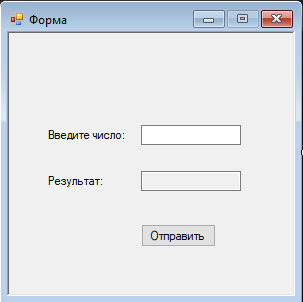
\includegraphics{task1/form.png}
    \caption{Внешний вид формы программы для вычисления факториала}
    \label{fig:task1_form}
\end{figure}
У элементов изменены значения некоторых атрибутов. 
Значения измененных атрибутов представлены в таблице \ref{table:params1}.

\begin{table}[H]
    \small
    \caption{Значения атрибутов элементов в приложении <<Факториал>>}
    \begin{tabular}{|l|l|}\hline
    Наименование атрибута & Значение\cr\hline
    \multicolumn{2}{|l|}{Для формы}\cr\hline
    \verb"Text" & \verb"Форма"\cr\hline
    \verb"FormBorderStyle" & \verb"FixedSingle"\cr\hline
    \verb"MaximizeBox" & \verb"False"\cr\hline
    \multicolumn{2}{|l|}{Для первой надписи}\cr\hline
    \verb"(Name)" & \verb"lblInput"\cr\hline
    \verb"Text" & \verb"Введите целое число"\cr\hline
    \multicolumn{2}{|l|}{Для второй надписи}\cr\hline
    \verb"(Name)" & \verb"lblOutput"\cr\hline
    \verb"Text" & \verb"Результат"\cr\hline
    \multicolumn{2}{|l|}{Для первого текстового поля}\cr\hline
    \verb"(Name)" & \verb"txtInput"\cr\hline
    \multicolumn{2}{|l|}{Для второго текстового поля}\cr\hline
    \verb"(Name)" & \verb"txtOutput"\cr\hline
    \multicolumn{2}{|l|}{Для кнопки}\cr\hline
    \verb"(Name)" & \verb"btnCalculate"\cr\hline
    \verb"Text" & \verb"Вычислить"\cr\hline
    \multicolumn{2}{|l|}{Для обработчика ошибок}\cr\hline
    \verb"(Name)" & \verb"errorProvider1"\cr\hline
    \end{tabular}
    \label{table:params1}
\end{table}

Для работы программы была написана функция вычисления факториала:
\inputminted[fontsize=\small, breaklines=true, style=bw, linenos]{cpp}{task1/fact.h}
Здесь переменная \verb|N| "--- число, для которого нужно вычислить факториал.

На нажатие кнопки <<Вычислить>> установлено выполнение следующего
кода:
\begin{minted}[fontsize=\small, breaklines=true, style=bw, linenos]{cpp}
    private: System::Void btnCalculate_Click(System::Object^ sender, System::EventArgs^ e) {
		ClearAll();
		ll InputNumber;
		bool result = Int64::TryParse(txtInput->Text, InputNumber);
		if (!result) {
			errorProvider1->SetError(txtInput, "Введено не целое число");
			return;
		}
		if (InputNumber > 20) {
			errorProvider1->SetError(txtInput, "Число слишком большое");
			return;
		}
		ll OutputNumber = fact(InputNumber);
		if (OutputNumber == -1) {
			errorProvider1->SetError(txtInput, "Введено отрицательное число");
			return;
		}
		txtOutput->Text = System::Convert::ToString(OutputNumber);
	}
\end{minted}

После запуска приложения на экране появляется окно (см. рисунок \ref{fig:exec1})
\begin{figure}[H]
    \centering
    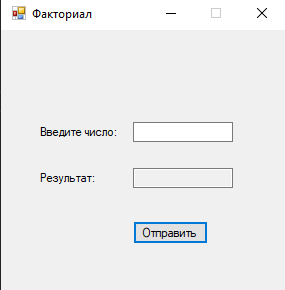
\includegraphics{task1/exec.png}
    \caption{Скриншот запуска программы}
    \label{fig:exec1}
\end{figure}

При вводе целого числа после нажатия кнопки в поле вывода приводится
результат вычисления факториала для заданного числа (см. рисунок \ref{fig:result1}).
\begin{figure}[H]
    \centering
    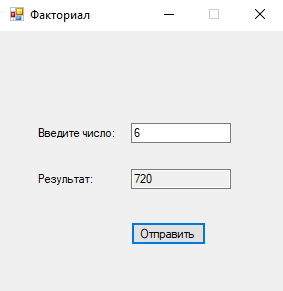
\includegraphics{task1/result.png}
    \caption{Результат работы}
    \label{fig:result1}
\end{figure}

Ввод некорректных значений обрабатывается элементом \verb|ErrorProvider| и 
сопровождается сообщением об ошибке (см. рисунок \ref{fig:error1} )
\begin{figure}[H]
    \centering
    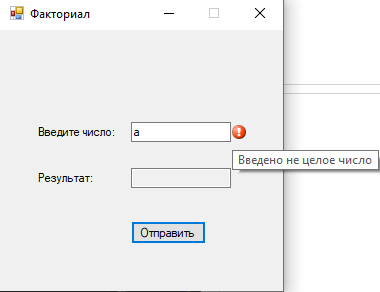
\includegraphics{task1/error.png}
    \caption{Сообщение об ошибке}
    \label{fig:error1}
\end{figure}
Полный код программы приведен в приложении \ref{app:repos}.
\section{Простые вычисления}

\textbf{Задание:} Вычислить значение выражения ~$\displaystyle \frac{\cos{x} + \sin{y}}{\ln(x + y)}$
\vspace{0.25cm}

Создано окно, содержащее три элемента \verb|TextBox|, три элемента \verb|Label| и 
один элемент \verb|Button|. Вид окна представлен на рисунке \ref{fig:form2}.

\begin{figure}[H]
    \centering
    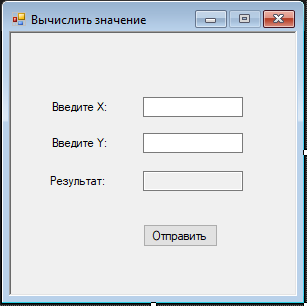
\includegraphics{task2/form.png}
    \caption{Внешний вид формы в конструкторе}
    \label{fig:form2}
\end{figure}

У элементов изменены значения некоторых атрибутов. 
Значения измененных атрибутов представлены в таблице \ref{table:params2}.

\begin{table}[H]
    \small
    \caption{Значения атрибутов элементов в приложении <<Простые вычисления>>}
    \begin{tabular}{|l|l|}\hline
    Наименование атрибута & Значение\cr\hline
    \multicolumn{2}{|l|}{Для формы}\cr\hline
    \verb"Text" & \verb"Вычислить значение"\cr\hline
    \verb"FormBorderStyle" & \verb"FixedSingle"\cr\hline
    \verb"MaximizeBox" & \verb"False"\cr\hline
    \multicolumn{2}{|l|}{Для первой надписи}\cr\hline
    \verb"(Name)" & \verb"xLabel"\cr\hline
    \verb"Text" & \verb"Введите X"\cr\hline
    \multicolumn{2}{|l|}{Для второй надписи}\cr\hline
    \verb"(Name)" & \verb"yLabel"\cr\hline
    \verb"Text" & \verb"Введите Y"\cr\hline
    \multicolumn{2}{|l|}{Для третьей надписи}\cr\hline
    \verb"(Name)" & \verb"lblOutput"\cr\hline
    \verb"Text" & \verb"Результат:"\cr\hline
    \multicolumn{2}{|l|}{Для первого текстового поля}\cr\hline
    \verb"(Name)" & \verb"xInput"\cr\hline
    \multicolumn{2}{|l|}{Для второго текстового поля}\cr\hline
    \verb"(Name)" & \verb"yInput"\cr\hline
    \multicolumn{2}{|l|}{Для третьего текстового поля}\cr\hline
    \verb"(Name)" & \verb"txtOutput"\cr\hline
    \multicolumn{2}{|l|}{Для кнопки}\cr\hline
    \verb"(Name)" & \verb"btnCalculate"\cr\hline
    \verb"Text" & \verb"Вычислить"\cr\hline
    \multicolumn{2}{|l|}{Для обработчика ошибок}\cr\hline
    \verb"(Name)" & \verb"errorProvider1"\cr\hline
    \end{tabular}
    \label{table:params2}
\end{table}

Для работы программы была написана функция вычисления заданного выражения:
\inputminted[fontsize=\small, breaklines=true, style=bw, linenos]{cpp}{task2/f.h}
и функция, проверяющая выбранное поле на корректность\cite{MS, MS1}:
\begin{minted}[fontsize=\small, breaklines=true, style=bw, linenos]{asm}
    bool VarValidation(System::Windows::Forms::TextBox^ Input, ll& x) { // Проверка числа для поля x из текста объекта Input
		
		ll InputNumber;
		bool IsVariableValid = Int64::TryParse(Input->Text, InputNumber); // Пробуем записать в InputNumber число из потока
		
		if (!IsVariableValid) { // Если не вышло
			errorProvider1->SetError(Input, "Переменная не целое число");
			return 0;
		}
		x = InputNumber; // Обновляем значение переменной
		return 1;
    }
\end{minted}
Логику работы программы реализует фрагмент кода, привязанный к кнопке
\begin{minted}[fontsize=\small, breaklines=true, style=bw, linenos]{cpp}
	private: System::Void btnCalculate_Click(System::Object^ sender, System::EventArgs^ e) {
		ClearAll();

		ll x = 0;
		ll y = 0;

		bool XisOkay = VarValidation(xInput, x); // Проверяем корректность x
		bool YisOkay = VarValidation(yInput, y); // Проверяем корректность y

		if (!XisOkay || !YisOkay) return; // Если какая-то из них некорректна - завершим работу. Все необходимые выводы исключений уже были произведены

		ll summary = x + y; // Считаем сумму для логарифма

		if (summary == 1) { // Если аргумент равен единице - логарифм равен нулю
			errorProvider1->SetError(txtOutput, "Деление на ноль");
			return;
		}

		if (summary <= 0) { // Если аргумент меньше нуля - неверно
			errorProvider1->SetError(txtOutput, "Недопустимое значение для логарифма");
			return;
		}

		double OutputNumber = f(x, y); // Получаем значение функции для заданных чисел х, у

		txtOutput->Text = System::Convert::ToString(OutputNumber); // Отображаем ответ
	}
\end{minted}

Функция \verb|ClearAll()| реализует очищение полей от ошибок.
После запуска приложения на экране появляется окно (см. рисунок \ref{fig:exec2})
\begin{figure}[H]
    \centering
    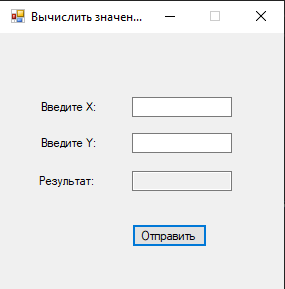
\includegraphics{task2/exec.png}
    \caption{Скриншот запуска программы}
    \label{fig:exec2}
\end{figure}
При вводе целого числа после нажатия кнопки в поле вывода приводится
результат вычисления факториала для заданного числа (см. рисунок \ref{fig:result2}).
\begin{figure}[H]
    \centering
    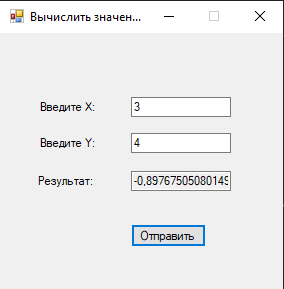
\includegraphics{task2/result.png}
    \caption{Результат работы}
    \label{fig:result2}
\end{figure}
Ввод некорректных значений обрабатывается элементом \verb|ErrorProvider| и 
сопровождается сообщением об ошибке (см. рисунок \ref{fig:error2} )
\begin{figure}[H]
    \centering
    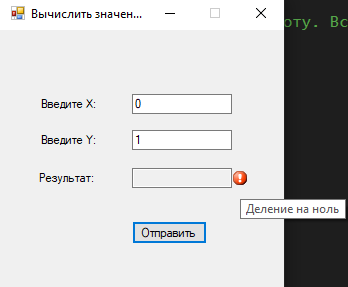
\includegraphics{task2/error.png}
    \caption{Сообщение об ошибке}
    \label{fig:error2}
\end{figure}
Полный код программы приведен в приложении \ref{app:repos}.
\section{Рекурсивные вычисления}
\textbf{Задание:} Создать рекурсивную функцию, которая для заданного целого $n$
вычисляет сумму ряда $\displaystyle \sum\limits_{i=1}^n 2^i$

Для этого были использовано 3 элемента \verb|Label|, 2 элемента \verb|TextBox|, 1 элемент \verb|PictureBox|
и один элемент \verb|Button|. 

Создано окно, содержащее три элемента \verb|TextBox|, три элемента \verb|Label| и 
один элемент \verb|Button|. После запуска приложения появляется окно (см. рисунок \ref{fig:form3}) .
\begin{figure}[H]
    \centering
    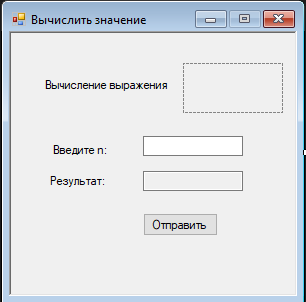
\includegraphics{task3/form.png}
    \caption{Внешний вид формы в конструкторе}
    \label{fig:form3}
\end{figure}
У элементов изменены значения некоторых атрибутов. 
Значения измененных атрибутов представлены в таблице \ref{table:params3}.
\begin{table}[H]
    \small
    \caption{Значения атрибутов элементов в приложении <<Рекурсивные вычисления>>}
    \begin{tabular}{|l|l|}\hline
    Наименование атрибута & Значение\cr\hline
    \multicolumn{2}{|l|}{Для формы}\cr\hline
    \verb"Text" & \verb"Вычислить значение"\cr\hline
    \verb"FormBorderStyle" & \verb"FixedSingle"\cr\hline
    \verb"MaximizeBox" & \verb"False"\cr\hline
    \multicolumn{2}{|l|}{Для первой надписи}\cr\hline
    \verb"(Name)" & \verb"formulaText"\cr\hline
    \verb"Text" & \verb"Вычисление выражения"\cr\hline
    \multicolumn{2}{|l|}{Для второй надписи}\cr\hline
    \verb"(Name)" & \verb"xLabel"\cr\hline
    \verb"Text" & \verb"Введите N"\cr\hline
    \multicolumn{2}{|l|}{Для третьей надписи}\cr\hline
    \verb"(Name)" & \verb"lblOutput"\cr\hline
    \verb"Text" & \verb"Результат:"\cr\hline
    \multicolumn{2}{|l|}{Для первого текстового поля}\cr\hline
    \verb"(Name)" & \verb"xInput"\cr\hline
    \multicolumn{2}{|l|}{Для второго текстового поля}\cr\hline
    \verb"(Name)" & \verb"txtOutput"\cr\hline
    \multicolumn{2}{|l|}{Для кнопки}\cr\hline
    \verb"(Name)" & \verb"btnCalculate"\cr\hline
    \verb"Text" & \verb"Вычислить"\cr\hline
    \multicolumn{2}{|l|}{Для обработчика ошибок}\cr\hline
    \verb"(Name)" & \verb"errorProvider1"\cr\hline
    \multicolumn{2}{|l|}{Для изображения выражения}\cr\hline
    \verb"(Name)" & \verb"pictureBox1"\cr\hline
    \end{tabular}
    \label{table:params3}
\end{table}
Программа содержит функции (\verb|ClearAll|, \verb|VarValidation|), 
аналогичные функциям в программе <<Простые вычисления>> за исключением логики работы кнопки:
\begin{minted}[fontsize=\small, breaklines=true, style=bw, linenos]{cpp}
    private: System::Void btnCalculate_Click(System::Object^ sender, System::EventArgs^ e) {
		ClearAll();

		ll n = 0;

		bool NisOkay = VarValidation(nInput, n); // Проверяем корректность n

		if (n <= 0) {
			errorProvider1->SetError(nInput, "Недопустимая степень");
			return;
		}
			

		if (!NisOkay) return; // Если число некорректно - завершим работу. Все необходимые выводы исключений уже были произведены

		ll OutputNumber = f(n); // Получаем значение ряда для заданного n

		txtOutput->Text = System::Convert::ToString(OutputNumber); // Отображаем ответ
	}
\end{minted}
и функции подсчета суммы ряда
\inputminted[fontsize=\small, breaklines=true, style=bw, linenos]{cpp}{task3/f.h}

Неверно введеннные данные обрабатываются элементом \verb|ErrorProvider|. 

Полный код программы представлен в приложении \ref{app:repos}.
\section{Обработка табличных данных. Часть 1.}

\textbf{Задание:} Найти сумму нечетных элементов, меньших заданного числа. 
Вывести максимальный четный элемент. 

Создано окно приложения, содержащее два элемента \verb|TextBox|, два элемента \verb|Label|, 
4 элемента \verb|Button|, и 1 элемент \verb|DataGridView|. 
Для отображения сообщений об ошибках в окно добавлен элемент \verb|ErrorProvider|. 
Вид окна представлен на рисунке \ref{fig:task4_form}.
\begin{figure}[H]
    \centering
    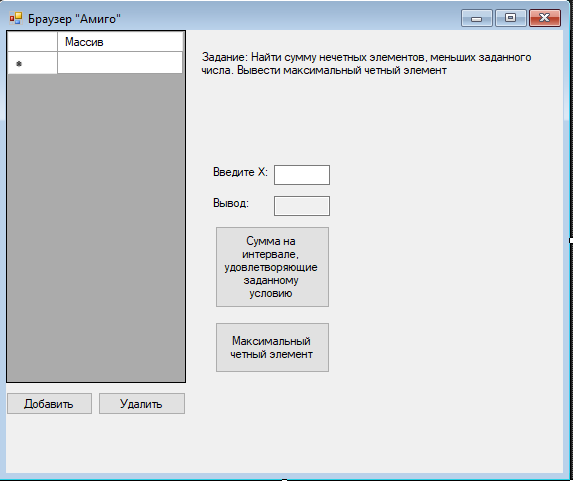
\includegraphics{task4/form.png}
    \caption{Внешний вид формы программы}
    \label{fig:task4_form}
\end{figure}
У элементов изменены значения некоторых атрибутов. 
Значения измененных атрибутов представлены в таблице \ref{table:params4}.
\begin{table}[H]
    \small
    \caption{Значения атрибутов элементов в приложении <<Обработка табличных данных. Часть 1.>>}
    \begin{tabular}{|l|l|}\hline
    Наименование атрибута & Значение\cr\hline
    \multicolumn{2}{|l|}{Для формы}\cr\hline
    \verb"Text" & \verb"Браузер "Амиго""\cr\hline
    \verb"FormBorderStyle" & \verb"FixedSingle"\cr\hline
    \verb"MaximizeBox" & \verb"False"\cr\hline
    \multicolumn{2}{|l|}{Для первой надписи}\cr\hline
    \verb"(Name)" & \verb"xLabel"\cr\hline
    \verb"Text" & \verb"Введите X"\cr\hline
    \multicolumn{2}{|l|}{Для второй надписи}\cr\hline
    \verb"(Name)" & \verb"lblOutput"\cr\hline
    \verb"Text" & \verb"Вывод"\cr\hline
    \multicolumn{2}{|l|}{Для первого текстового поля}\cr\hline
    \verb"(Name)" & \verb"txtX"\cr\hline
    \multicolumn{2}{|l|}{Для второго текстового поля}\cr\hline
    \verb"(Name)" & \verb"txtOutput"\cr\hline
    \multicolumn{2}{|l|}{Для кнопки суммирования}\cr\hline
    \verb"(Name)" & \verb"btnSummary"\cr\hline
    \verb"Text" & \verb"Сумма на интервале, удовлетворяющие заданному условию"\cr\hline
    \multicolumn{2}{|l|}{Для кнопки для нахождения максимального четного элемента}\cr\hline
    \verb"(Name)" & \verb"btnFindMaxEven"\cr\hline
    \verb"Text" & \verb"Максимальный четный элемент"\cr\hline
    \multicolumn{2}{|l|}{Для кнопки для нахождения максимального четного элемента}\cr\hline
    \verb"(Name)" & \verb"btnFindMaxEven"\cr\hline
    \verb"Text" & \verb"Максимальный четный элемент"\cr\hline
    \multicolumn{2}{|l|}{Для кнопки добавления ряда}\cr\hline
    \verb"(Name)" & \verb"btnAdd"\cr\hline
    \verb"Text" & \verb"Добавить"\cr\hline
    \multicolumn{2}{|l|}{Для кнопки удаления ряда}\cr\hline
    \verb"(Name)" & \verb"btnRemove"\cr\hline
    \verb"Text" & \verb"Удалить"\cr\hline
    \multicolumn{2}{|l|}{Для таблицы}\cr\hline
    \verb"(Name)" & \verb"grid"\cr\hline
    \verb"(Name)" & \verb"grid"\cr\hline
    \multicolumn{2}{|l|}{Для обработчика ошибок}\cr\hline
    \verb"(Name)" & \verb"errorProvider1"\cr\hline
    \end{tabular}
    \label{table:params4}
\end{table}
Для изменения количества рядов в таблице были реализованы кнопки добавления
и удаления ряда. Код соответствующих функций приведен ниже:
\begin{minted}[fontsize=\small, breaklines=true, style=bw, linenos]{cpp}
    private: System::Void btnAdd_Click(System::Object^ sender, System::EventArgs^ e) { // Добавление
			this->grid->Rows->Add(1);
	}
    private: System::Void btnRemove_Click(System::Object^ sender, System::EventArgs^ e) { // Удаление
		if (!this->grid->CurrentRow->IsNewRow) {
			int i = this->grid->CurrentRow->Index;
			this->grid->Rows->Remove(this->grid->Rows[i]);
		}
	}

\end{minted}
Решение каждой из двух задач реализовано в соответствующих кнопках. Код 
представлен ниже:
\begin{minted}[fontsize=\footnotesize, breaklines=true, style=bw, linenos]{cpp}
private: System::Void btnSummary_Click(System::Object^ sender, System::EventArgs^ e) { // Вычисление необходимой суммы
	ClearOutput();
	bool noBadCells = true;
	bool check2 = true;
	if ((int)WrongCells->size() > 0) {
		noBadCells = false;
	}
	int xValue;
	bool isCorrectValue = Int32::TryParse(txtX->Text, xValue);
	if (!isCorrectValue) {
		errorProvider1->SetError(txtX, "Неверное значение для X");
	}
	if (!isCorrectValue) {
		return;
	}
	else {
		errorProvider1->SetError(txtX, String::Empty);
	}
	if (!noBadCells) {
		return;
	}
	int summary = 0;
	for (int i = 0; i < this->grid->RowCount; ++i) {
		int val = System::Convert::ToInt32(this->grid->Rows[i]->Cells[0]->Value);
		if (val % 2 == 1 && val < xValue) {
			summary += val;
		}
	}
	ClearOutput();
	txtOutput->Text = System::Convert::ToString(summary);
	}
private: System::Void btnFindMaxEven_Click(System::Object^ sender, System::EventArgs^ e) { // Вывод необходимого максимального элемента на экран
	ClearOutput();
	if (WrongCells->size() > 0) {
		return;
	}
	int max_val = -1e9;
	int max_ind = -1;
	for (int i = 0; i < this->grid->RowCount; ++i) {
		int val = System::Convert::ToInt32(this->grid->Rows[i]->Cells[0]->Value);
		if (val > max_val && val % 2 == 0) {
			max_val = val;
			max_ind = i;
		}
	}
	ClearOutput();
	txtOutput->Text = System::Convert::ToString(max_val);
}
\end{minted}
Контроль за корректностью введенных данных осуществляется через поддерживание
невалидных ячеек в set из библиотеки STL. Работа с ней осуществляется через 
обработку события \verb|CellLeave|\cite{STL, BN, Kon, MS1}:
\begin{minted}[fontsize=\footnotesize, breaklines=true, style=bw, linenos]{cpp}
private: System::Void grid_CellLeave(System::Object^ sender, System::Windows::Forms::DataGridViewCellEventArgs^ e) {
	int val = 0;

	System::String^ Value = System::Convert::ToString(
		this->grid->Rows[grid->CurrentRow->Index]->Cells[0]->EditedFormattedValue);
			
	bool isCorrectValue = Int32::TryParse(Value, val); // Пробуем записать в InputNumber число из потока
	if (!isCorrectValue && (Value != "" && grid->CurrentRow->Index != grid->RowCount)) {
		errorProvider1->SetError(grid, "Неверный тип для ячейки");
		WrongCells->insert(grid->CurrentRow->Index);
	}
	else {
		WrongCells->erase(grid->CurrentRow->Index);
		if ((int)WrongCells->size() == 0) {
			errorProvider1->SetError(grid, String::Empty);
		}
	}	
}
\end{minted}
После запуска приложения на экране появляется окно (см. рисунок \ref{fig:exec4})
\begin{figure}[H]
    \centering
    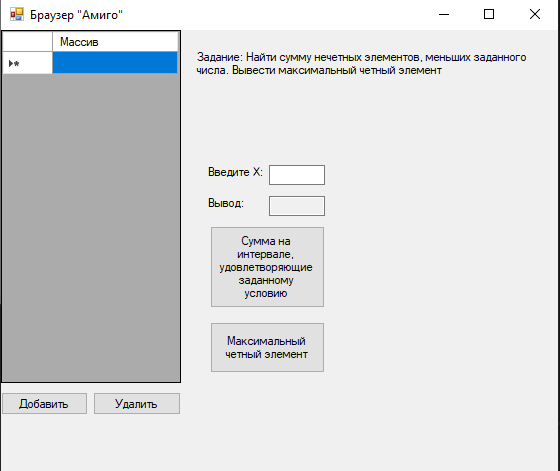
\includegraphics{task4/exec.png}
    \caption{Скриншот запуска программы}
    \label{fig:exec4}
\end{figure}
При вводе целого числа после нажатия кнопки в поле вывода приводится
результат вычисления суммы в заданном интервале (см. рисунок \ref{fig:result41}).
\begin{figure}[H]
    \centering
    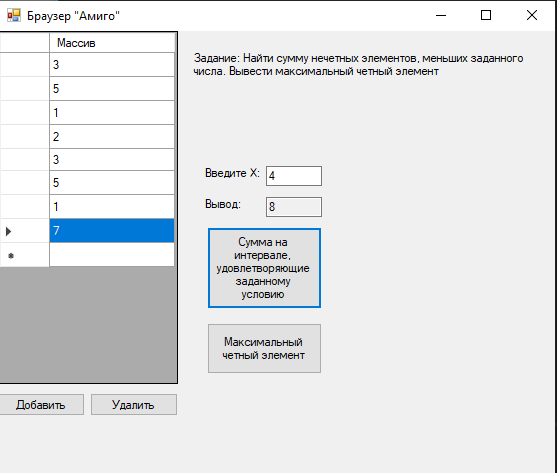
\includegraphics{task4/result1.png}
    \caption{Результат работы}
    \label{fig:result41}
\end{figure}
При вводе целого числа после нажатия кнопки в поле вывода приводится
результат вычисления максимального четного элемента (см. рисунок \ref{fig:result42}).
\begin{figure}[H]
    \centering
    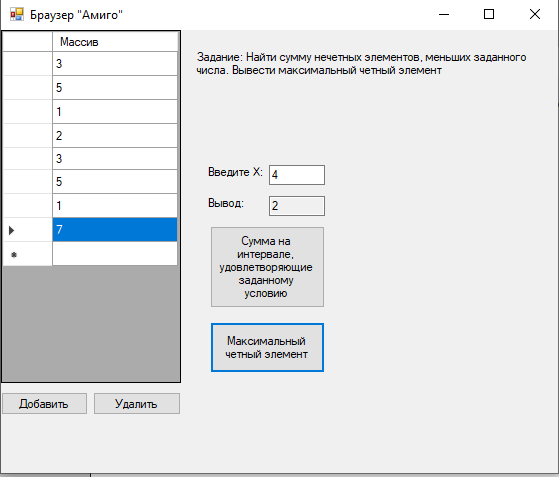
\includegraphics{task4/result2.png}
    \caption{Результат работы}
    \label{fig:result42}
\end{figure}
Ввод некорректных значений обрабатывается элементом \verb|ErrorProvider| и 
сопровождается сообщением об ошибке (см. рисунок \ref{fig:error4} )
\begin{figure}[H]
    \centering
    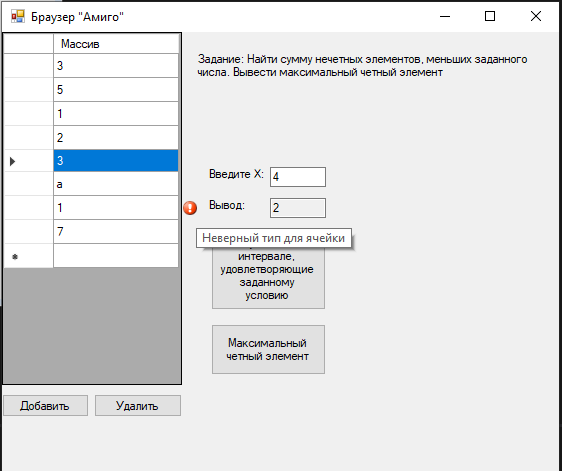
\includegraphics{task4/error.png}
    \caption{Сообщение об ошибке}
    \label{fig:error4}
\end{figure}
Полный код программы приведен в приложении \ref{app:repos}.
\section{Обработка табличных данных. Часть 2.}

\textbf{Задание:} Ваш выбор: Все нечетные столбцы заменить столбцом X. 
(Нумерация столбцов массива начинается с нуля.)

Создано окно приложения, содержащее 5 элементов \verb|Button|, 3 элемента \verb|DataGridView| 
и 5 элементов \verb|Label|. 
Для отображения сообщений об ошибках в окно добавлен элемент \verb|ErrorProvider|. 
Вид окна представлен на рисунке \ref{fig:task5_form}.
\begin{figure}[H]
    \centering
    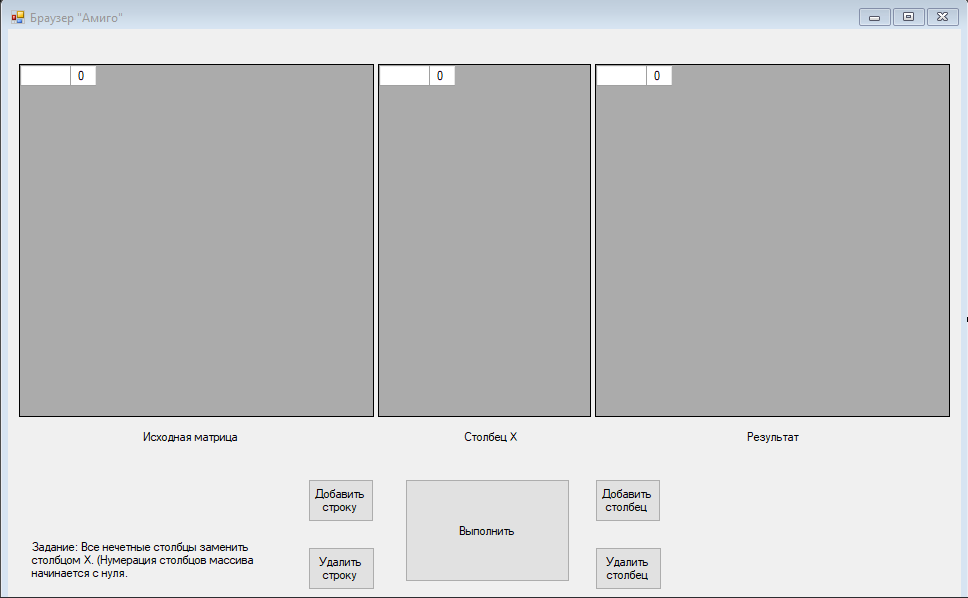
\includegraphics[scale=0.6]{task5/form.png}
    \caption{Внешний вид формы программы}
    \label{fig:task5_form}
\end{figure}
У элементов изменены значения некоторых атрибутов. 
Значения измененных атрибутов представлены в таблице \ref{table:params5}.
\begin{table}[H]
    \small
    \caption{Значения атрибутов элементов в приложении <<Обработка табличных данных. Часть 2.>>}
    \begin{tabular}{|l|l|}\hline
    Наименование атрибута & Значение\cr\hline
    \multicolumn{2}{|l|}{Для формы}\cr\hline
    \verb"Text" & \verb"Браузер "Амиго""\cr\hline
    \verb"FormBorderStyle" & \verb"FixedSingle"\cr\hline
    \verb"MaximizeBox" & \verb"False"\cr\hline
    \multicolumn{2}{|l|}{Для первой надписи}\cr\hline
    \verb"(Name)" & \verb"taskLabel"\cr\hline
    \verb"Text" & \verb"Задание: Все нечетные столбцы заменить столбцом X."\cr\hline
    \multicolumn{2}{|l|}{Для второй надписи}\cr\hline
    \verb"(Name)" & \verb"initLabel"\cr\hline
    \verb"Text" & \verb"Исходная матрица"\cr\hline
    \multicolumn{2}{|l|}{Для третьей надписи}\cr\hline
    \verb"(Name)" & \verb"xLabel"\cr\hline
    \verb"Text" & \verb"Столбец X"\cr\hline
    \multicolumn{2}{|l|}{Для четвертой надписи}\cr\hline
    \verb"(Name)" & \verb"resultLabel"\cr\hline
    \verb"Text" & \verb"Результат"\cr\hline
    \multicolumn{2}{|l|}{Для кнопки "Выполнить"}\cr\hline
    \verb"(Name)" & \verb"btnCalc"\cr\hline
    \multicolumn{2}{|l|}{Для кнопки добавления ряда}\cr\hline
    \verb"(Name)" & \verb"btnAddRow"\cr\hline
    \verb"Text" & \verb"Добавить"\cr\hline
    \multicolumn{2}{|l|}{Для кнопки удаления ряда}\cr\hline
    \verb"(Name)" & \verb"btnRemoveRow"\cr\hline
    \verb"Text" & \verb"Удалить"\cr\hline
    \multicolumn{2}{|l|}{Для кнопки добавления столбца}\cr\hline
    \verb"(Name)" & \verb"btnAddColumn"\cr\hline
    \verb"Text" & \verb"Добавить"\cr\hline
    \multicolumn{2}{|l|}{Для кнопки удаления столбца}\cr\hline
    \verb"(Name)" & \verb"btnRemoveColumn"\cr\hline
    \verb"Text" & \verb"Удалить"\cr\hline
    \multicolumn{2}{|l|}{Для обработчика ошибок}\cr\hline
    \verb"(Name)" & \verb"errorProvider1"\cr\hline
    \end{tabular}
    \label{table:params5}
\end{table}

После запуска приложения на экране появляется окно (см. рисунок \ref{fig:exec5})
\begin{figure}[H]
    \centering
    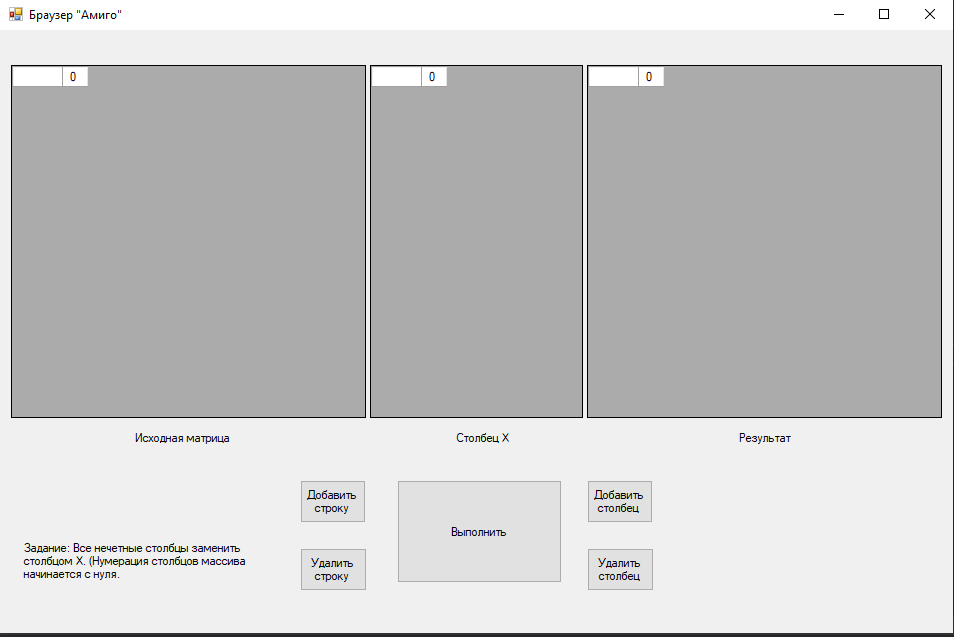
\includegraphics[scale=0.6]{task5/exec.png}
    \caption{Скриншот запуска программы}
    \label{fig:exec5}
\end{figure}
При вводе целого числа после нажатия кнопки в поле вывода приводится
результат вычисления суммы в заданном интервале (см. рисунок \ref{fig:result5}).
\begin{figure}[H]
    \centering
    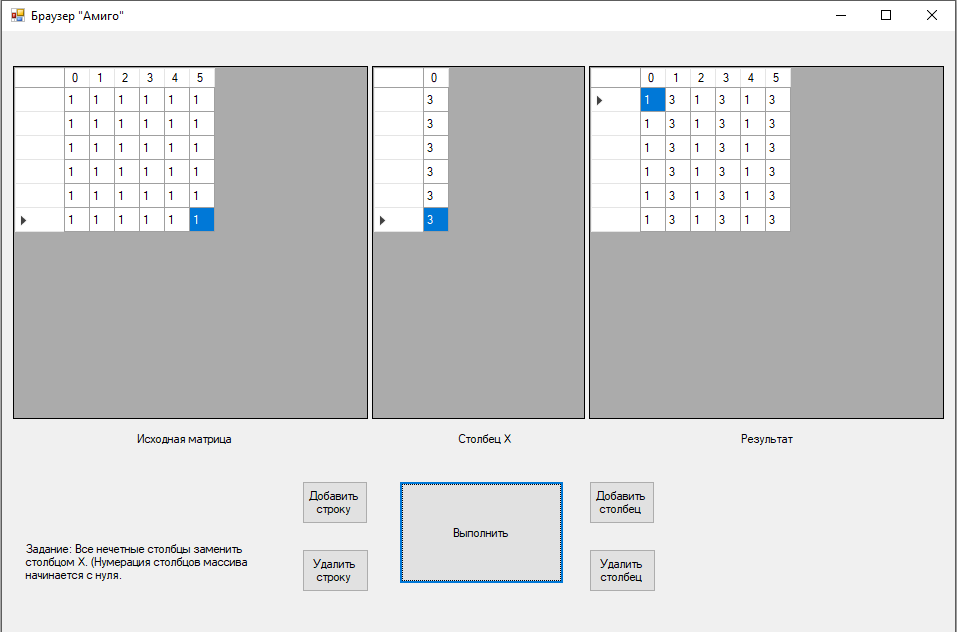
\includegraphics[scale=0.6]{task5/result.png}
    \caption{Результат работы}
    \label{fig:result5}
\end{figure}
Ввод некорректных значений обрабатывается элементом \verb|ErrorProvider| и 
сопровождается сообщением об ошибке (см. рисунок \ref{fig:error5} )
\begin{figure}[H]
    \centering
    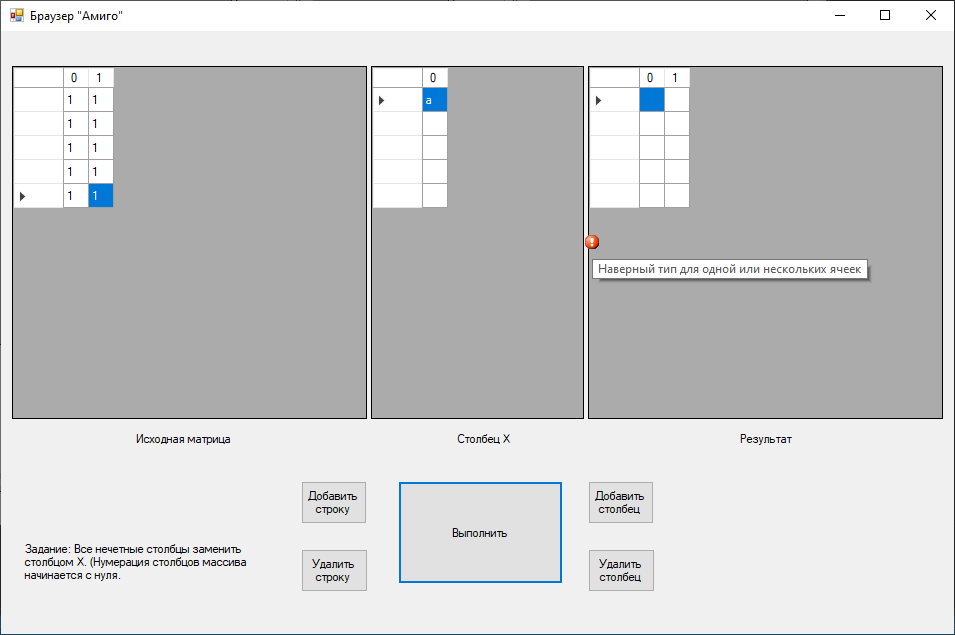
\includegraphics[scale=0.45]{task5/error.png}
    \caption{Сообщение об ошибке}
    \label{fig:error5}
\end{figure}
Полный код программы приведен в приложении \ref{app:repos}.
\section{Матричный калькулятор}
\textbf{Задание:} Создать приложение, реализующее основные операции с векторами и матрицами:

\begin{enumerate}
    \item Ввод матрицы, вектора
    \item Создание матриц (единичная, матрица как набор векторов)
    \item Умножение на число, вектор, матрицу
    \item Сложение/вычитание двух матриц
    \item Сложение/вычитание двух векторов
    \item Скалярное и векторное произведение двух векторов
    \item Транспонированная матрица
    \item Определитель, ранг матрицы
\end{enumerate}
Выводить сообщения об ошибках (ввод не числа, несоответствие размерностей)


Всего приложение  содержит 11 элементов \verb|Button|, 13 элементов \verb|RadioButton|,
5 элементов \verb|Label|, 4 элемента \verb|TextBox| и 3 элемента \verb|DataGridView|.


Интерфейс приложения можно условно разделить на четыре части, две из которых
отвечают за определение соответствующих аргументов операции, третья
за непосредственно саму операцию, а четвертая графически отображает
аргументы и результат
Вид окна представлен на рисунке \ref{fig:task6_form}.
\begin{figure}[H]
    \centering
    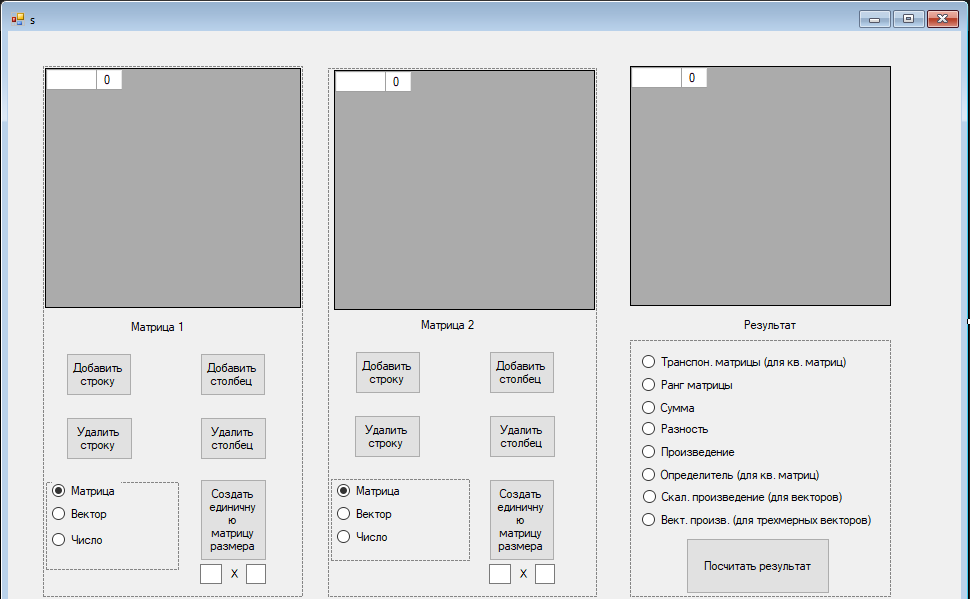
\includegraphics[scale=0.7]{task6/form.png}
    \caption{Внешний вид формы программы}
    \label{fig:task6_form}
\end{figure}
У элементов изменены значения некоторых атрибутов. 
Значения измененных атрибутов представлены в таблице \ref{table:params6}.
\begin{longtable}{|l|l|}
    Наименование атрибута & Значение\cr\hline
    \multicolumn{2}{|l|}{Для формы}\cr\hline
    \verb"Text" & \verb"Браузер "Амиго""\cr\hline
    \verb"FormBorderStyle" & \verb"FixedSingle"\cr\hline
    \verb"MaximizeBox" & \verb"False"\cr\hline
    \multicolumn{2}{|l|}{Для первой группы}\cr\hline
    \verb"(Name)" & \verb"MatrixGroup1"\cr\hline
    \multicolumn{2}{|l|}{Для второй группы}\cr\hline
    \verb"(Name)" & \verb"MatrixGroup2"\cr\hline
    \multicolumn{2}{|l|}{Для третьей группы}\cr\hline
    \verb"(Name)" & \verb"Result_Group"\cr\hline
    \multicolumn{2}{|l|}{Для надписи первой матрицы}\cr\hline
    \verb"(Name)" & \verb"initLabel"\cr\hline
    \verb"Text" & \verb"Матрица 1"\cr\hline
    \multicolumn{2}{|l|}{Для надписи второй матрицы}\cr\hline
    \verb"(Name)" & \verb"xLabel"\cr\hline
    \verb"Text" & \verb"Матрица 2"\cr\hline
    \multicolumn{2}{|l|}{Для третьей надписи}\cr\hline
    \verb"(Name)" & \verb"resultLabel"\cr\hline
    \verb"Text" & \verb"Результат"\cr\hline
    \multicolumn{2}{|l|}{Для радиокнопки "Матрица" для группы 1}\cr\hline
    \verb"(Name)" & \verb"Grid1_MatrixRBtn"\cr\hline
    \verb"Text" & \verb"Матрица"\cr\hline
    \multicolumn{2}{|l|}{Для радиокнопки "Вектор" для группы 1}\cr\hline
    \verb"(Name)" & \verb"Grid1_VectorRBtn"\cr\hline
    \verb"Text" & \verb"Вектор"\cr\hline
    \multicolumn{2}{|l|}{Для радиокнопки "Число" для группы 1}\cr\hline
    \verb"(Name)" & \verb"Grid1_NumRBtn"\cr\hline
    \verb"Text" & \verb"Число"\cr\hline
    \multicolumn{2}{|l|}{Для радиокнопки "Матрица" для группы 2}\cr\hline
    \verb"(Name)" & \verb"Grid2_MatrixRBtn"\cr\hline
    \verb"Text" & \verb"Матрица"\cr\hline
    \multicolumn{2}{|l|}{Для радиокнопки "Вектор" для группы 2}\cr\hline
    \verb"(Name)" & \verb"Grid2_VectorRBtn"\cr\hline
    \verb"Text" & \verb"Вектор"\cr\hline
    \multicolumn{2}{|l|}{Для радиокнопки "Число" для группы 2}\cr\hline
    \verb"(Name)" & \verb"Grid2_NumRBtn"\cr\hline
    \verb"Text" & \verb"Число"\cr\hline
    \multicolumn{2}{|l|}{Для радиокнопки транспонирования для группы 3}\cr\hline
    \verb"(Name)" & \verb"Transposition_RBtn"\cr\hline
    \verb"Text" & \verb"Транспон. матрицы (для кв. матриц)"\cr\hline
    \multicolumn{2}{|l|}{Для радиокнопки ранга матрицы для группы 3}\cr\hline
    \verb"(Name)" & \verb"Rank_RBtn"\cr\hline
    \verb"Text" & \verb"Ранг матрицы"\cr\hline
    \multicolumn{2}{|l|}{Для радиокнопки суммы для группы 3}\cr\hline
    \verb"(Name)" & \verb"Sum_RBtn"\cr\hline
    \verb"Text" & \verb"Сумма"\cr\hline
    \multicolumn{2}{|l|}{Для радиокнопки разности для группы 3}\cr\hline
    \verb"(Name)" & \verb"Difference_RBtn"\cr\hline
    \verb"Text" & \verb"Разность"\cr\hline
    \multicolumn{2}{|l|}{Для радиокнопки произведения для группы 3}\cr\hline
    \verb"(Name)" & \verb"Mult_RBtn"\cr\hline
    \verb"Text" & \verb"Произведение"\cr\hline
    \multicolumn{2}{|l|}{Для радиокнопки определителя для группы 3}\cr\hline
    \verb"(Name)" & \verb"Det_RBtn"\cr\hline
    \verb"Text" & \verb"Определитель (для кв. матриц) "\cr\hline
    \multicolumn{2}{|l|}{Для радиокнопки скалярного произведения для группы 3}\cr\hline
    \verb"(Name)" & \verb"ScalarMultiply_RBtn"\cr\hline
    \verb"Text" & \verb"Скалярное произведение (для векторов) "\cr\hline
    \multicolumn{2}{|l|}{Для радиокнопки векторного произведения для группы 3}\cr\hline
    \verb"(Name)" & \verb"VectorMultiply_RBtn"\cr\hline
    \verb"Text" & \verb"Векторное произведение (для трехмерных векторов)"\cr\hline
    \multicolumn{2}{|l|}{Для кнопки создания единичной матрицы для группы 1}\cr\hline
    \verb"(Name)" & \verb"CreateMatrix1_Btn"\cr\hline
    \verb"Text" & \verb"Создать единичную матрицу размера"\cr\hline
    \multicolumn{2}{|l|}{Для кнопки создания единичной матрицы для группы 2}\cr\hline
    \verb"(Name)" & \verb"CreateMatrix2_Btn"\cr\hline
    \verb"Text" & \verb"Создать единичную матрицу размера"\cr\hline
    \multicolumn{2}{|l|}{Для знака размерности для группы 1}\cr\hline
    \verb"(Name)" & \verb"Scale_label1"\cr\hline
    \verb"Text" & \verb"X"\cr\hline
    \multicolumn{2}{|l|}{Для знака размерности для группы 2}\cr\hline
    \verb"(Name)" & \verb"Scale_label2"\cr\hline
    \verb"Text" & \verb"X"\cr\hline
    \multicolumn{2}{|l|}{Для текстового поля N размерности для группы 1}\cr\hline
    \verb"(Name)" & \verb"N1_TextBox"\cr\hline
    \multicolumn{2}{|l|}{Для текстового поля M размерности для группы 1}\cr\hline
    \verb"(Name)" & \verb"M1_TextBox"\cr\hline
    \multicolumn{2}{|l|}{Для текстового поля N размерности для группы 2}\cr\hline
    \verb"(Name)" & \verb"N2_TextBox"\cr\hline
    \multicolumn{2}{|l|}{Для текстового поля M размерности для группы 2}\cr\hline
    \verb"(Name)" & \verb"M2_TextBox"\cr\hline
    \multicolumn{2}{|l|}{Для кнопки "Добавить строку" для группы 1}\cr\hline
    \verb"(Name)" & \verb"Grid1_btnAddRow"\cr\hline
    \verb"Text" & \verb"Добавить строку"\cr\hline
    \multicolumn{2}{|l|}{Для кнопки "Добавить столбец" для группы 1}\cr\hline
    \verb"(Name)" & \verb"Grid1_btnAddColumn"\cr\hline
    \verb"Text" & \verb"Добавить столбец"\cr\hline
    \multicolumn{2}{|l|}{Для кнопки "Удалить строку" для группы 1}\cr\hline
    \verb"(Name)" & \verb"Grid1_btnRmvRow"\cr\hline
    \verb"Text" & \verb"Удалить строку"\cr\hline
    \multicolumn{2}{|l|}{Для кнопки "Удалить столбец" для группы 1}\cr\hline
    \verb"(Name)" & \verb"Grid1_btnRmvColumn"\cr\hline
    \verb"Text" & \verb"Удалить столбец"\cr\hline
    \multicolumn{2}{|l|}{Для кнопки "Добавить строку" для группы 2}\cr\hline
    \verb"(Name)" & \verb"Grid2_btnAddRow"\cr\hline
    \verb"Text" & \verb"Добавить строку"\cr\hline
    \multicolumn{2}{|l|}{Для кнопки "Добавить столбец" для группы 2}\cr\hline
    \verb"(Name)" & \verb"Grid2_btnAddColumn"\cr\hline
    \verb"Text" & \verb"Добавить столбец"\cr\hline
    \multicolumn{2}{|l|}{Для кнопки "Удалить строку" для группы 2}\cr\hline
    \verb"(Name)" & \verb"Grid2_btnRmvRow"\cr\hline
    \verb"Text" & \verb"Удалить строку"\cr\hline
    \multicolumn{2}{|l|}{Для кнопки "Удалить столбец" для группы 2}\cr\hline
    \verb"(Name)" & \verb"Grid2_btnRmvColumn"\cr\hline
    \verb"Text" & \verb"Удалить столбец"\cr\hline
    \multicolumn{2}{|l|}{Для кнопки добавления ряда}\cr\hline
    \verb"(Name)" & \verb"btnAddRow"\cr\hline
    \verb"Text" & \verb"Добавить"\cr\hline
    \multicolumn{2}{|l|}{Для кнопки удаления ряда}\cr\hline
    \verb"(Name)" & \verb"btnRemoveRow"\cr\hline
    \verb"Text" & \verb"Удалить"\cr\hline
    \multicolumn{2}{|l|}{Для кнопки добавления столбца}\cr\hline
    \verb"(Name)" & \verb"btnAddColumn"\cr\hline
    \verb"Text" & \verb"Добавить"\cr\hline
    \multicolumn{2}{|l|}{Для кнопки удаления столбца}\cr\hline
    \verb"(Name)" & \verb"btnRemoveColumn"\cr\hline
    \verb"Text" & \verb"Удалить"\cr\hline
    \multicolumn{2}{|l|}{Для обработчика ошибок}\cr\hline
    \verb"(Name)" & \verb"errorProvider1"\cr\hline
    \caption{Значения атрибутов элементов в приложении <<Матричный калькулятор}
    \label{table:params6}
\end{longtable}
Программа работает за счет дополнительно написанной библиотеки для работы с матрицами 
с помощью \verb|std::vector| библиотеки \verb|STL|. В ней реализованы все операции.
Код этой работы содержится в приложении А\cite{matrix, Boris, Sed, Iv}.

Кроме того, написаны две вспомогательный функции, представляющие из себя связки
между \verb|std::vector| и \verb|DataGridView|. Код приведен ниже:
\inputminted[fontsize=\small, breaklines=true, style=bw, linenos, encoding=cp1251, outencoding=utf8]{cpp}{task6/Misc.h}
Работа программы продемонстрирована на рисунках \ref{fig:det},\ref{fig:vec},\ref{fig:scalar}
\begin{figure}[H]
    \centering
    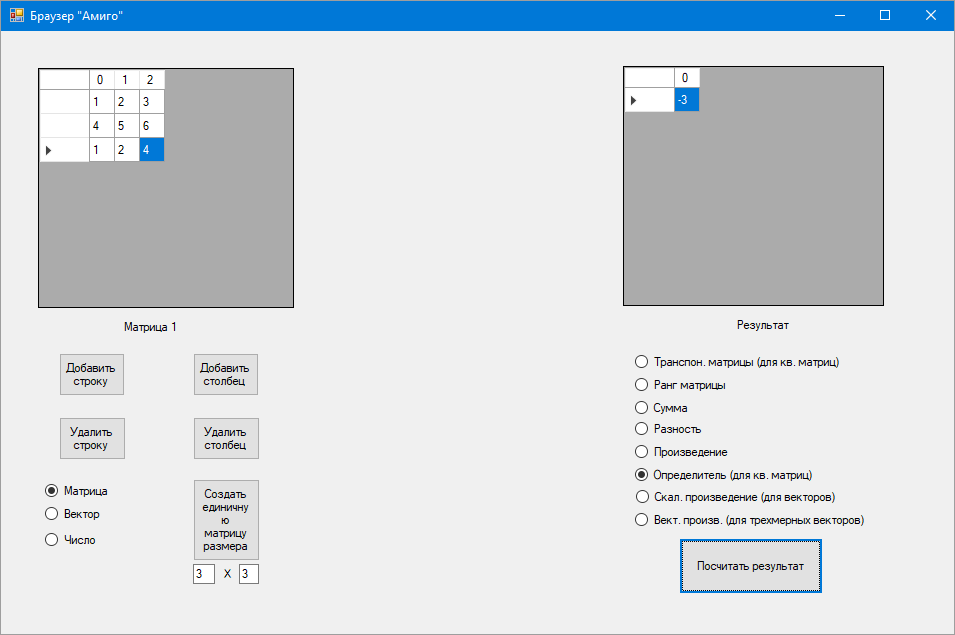
\includegraphics[scale=0.4]{task6/det.png}
    \caption{Пример нахождения определителя матрицы}
    \label{fig:det}
\end{figure}
\begin{figure}[H]
    \centering
    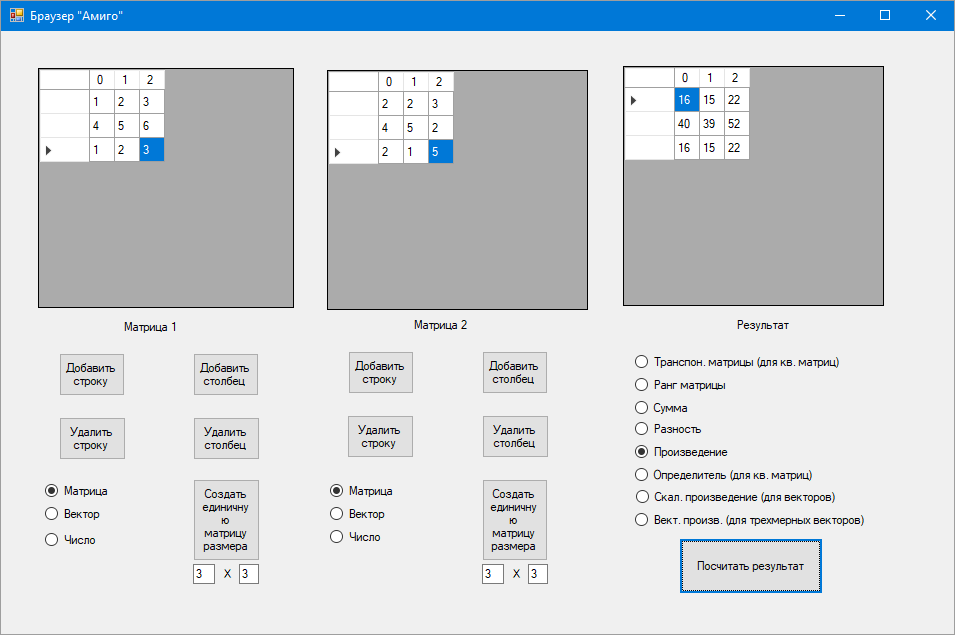
\includegraphics[scale=0.4]{task6/mult.png}   
    \caption{Пример нахождения векторного произведения}
    \label{fig:vec}
\end{figure}
\begin{figure}[H]
    \centering
    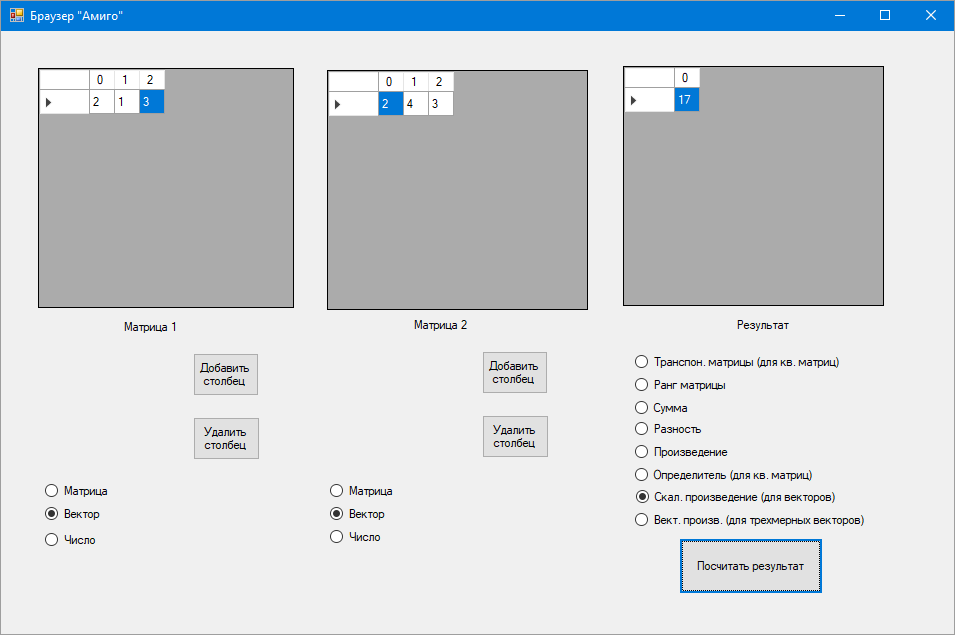
\includegraphics[scale=0.4]{task6/scalar.png}
    \caption{Пример нахождения скалярного произведения векторов}
    \label{fig:scalar}
\end{figure}

Можно заметить, что интерфейс приложения динамически изменяется в 
зависимости от выбранных параметров в соответствующих радиокнопках\cite{Pan}.

Контроль за корректностью введенных данных осуществляется внутри соответствующих
функций с помощью элемента \verb|ErrorProvider|. 

В случае, если вводятся некорректные данные или операция не поддерживается
над операндами этого типа "--- будет выведено сообщение об ошибке (см. рисунок \ref{fig:error6})
\begin{figure}[H]
    \centering
    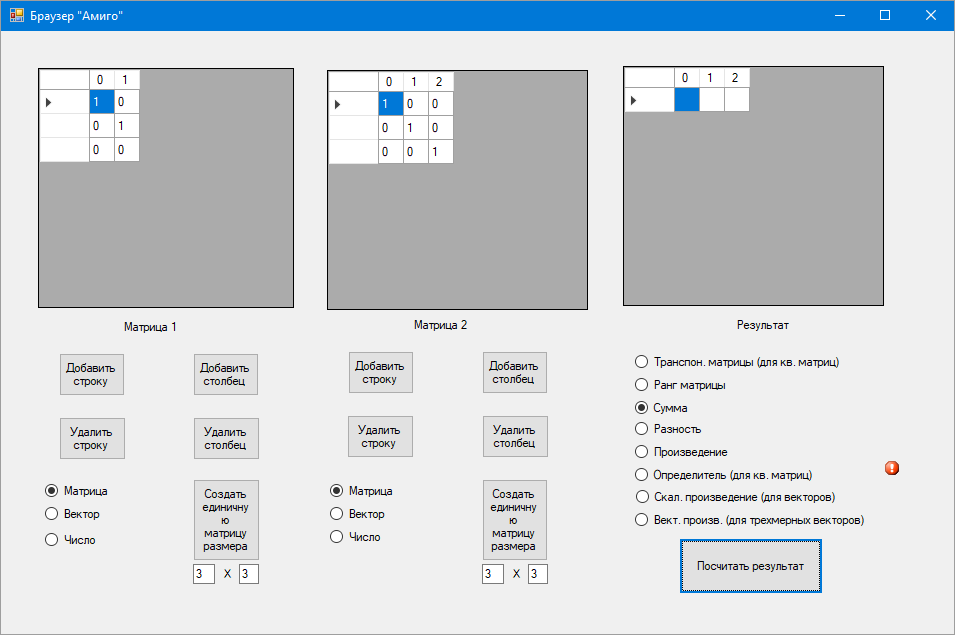
\includegraphics[scale=0.4]{task6/error1.png}
    \caption{Пример обработки ошибки}
    \label{fig:error6}
\end{figure}
Полный код программы приведен в приложении \ref{app:repos}.


\section{Использование коллекций}

\textbf{Задание:} Создать словарь, состоящий из строк. В качестве ключа выступает фамилия, в качестве значения "--- должность. Вывести на экран фамилии людей, занимающих данную должность. 
Вывести должность, занимаемую данным человеком.
Вид окна представлен на рисунке \ref{fig:task7_form}.
\begin{figure}[H]
    \centering
    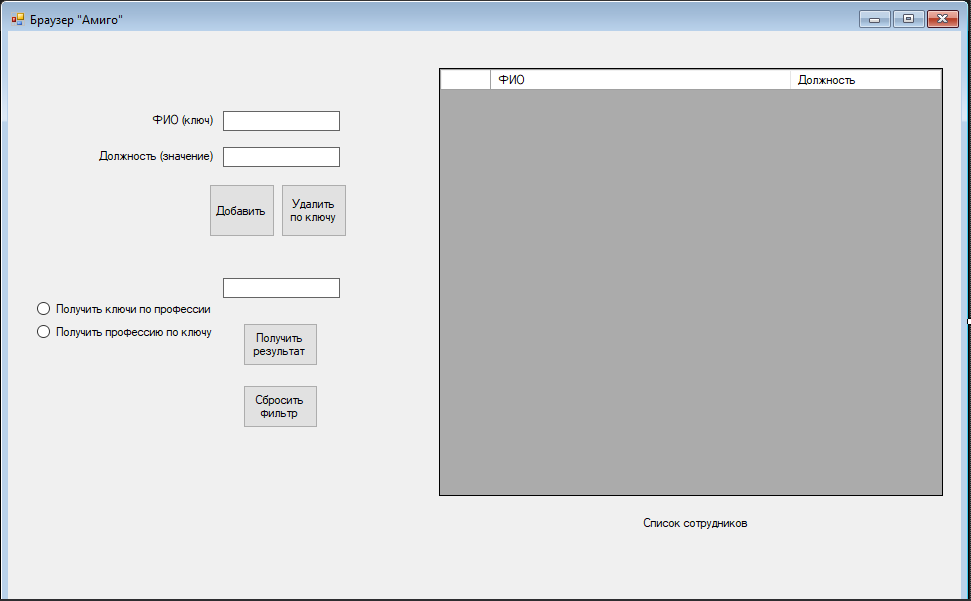
\includegraphics[scale=0.7]{task7/form.png}
    \caption{Внешний вид формы программы}
    \label{fig:task7_form}
\end{figure}
У элементов изменены значения некоторых атрибутов. 
Значения измененных атрибутов представлены в таблице \ref{table:params7}.
\begin{longtable}{|l|l|}
    Наименование атрибута & Значение\cr\hline
    \multicolumn{2}{|l|}{Для формы}\cr\hline
    \verb"Text" & \verb"Браузер "Амиго""\cr\hline
    \verb"FormBorderStyle" & \verb"FixedSingle"\cr\hline
    \verb"MaximizeBox" & \verb"False"\cr\hline
    \multicolumn{2}{|l|}{Для надписи ФИО}\cr\hline
    \verb"(Name)" & \verb"NameLabel"\cr\hline
    \verb"Text" & \verb"ФИО (ключ)"\cr\hline
    \multicolumn{2}{|l|}{Для текстового поля должности}\cr\hline
    \verb"(Name)" & \verb"PositionTextBox"\cr\hline
    \multicolumn{2}{|l|}{Для текстового поля ФИО}\cr\hline
    \verb"(Name)" & \verb"NameTextBox"\cr\hline
    \multicolumn{2}{|l|}{Для надписи должности}\cr\hline
    \verb"(Name)" & \verb"PositionLabel"\cr\hline
    \verb"Text" & \verb"Должность(значение)"\cr\hline
    \multicolumn{2}{|l|}{Для надписи к таблице}\cr\hline
    \verb"(Name)" & \verb"resultLabel"\cr\hline
    \verb"Text" & \verb"Список сотрудников"\cr\hline
    \multicolumn{2}{|l|}{Для кнопки добавления значения по ключу}\cr\hline
    \verb"(Name)" & \verb"AddBtn"\cr\hline
    \verb"Text" & \verb"Добавить"\cr\hline
    \multicolumn{2}{|l|}{Для кнопки удаления значения по ключу}\cr\hline
    \verb"(Name)" & \verb"RemoveBtn"\cr\hline
    \verb"Text" & \verb"Добавить"\cr\hline
    \multicolumn{2}{|l|}{Для текстового поля результата}\cr\hline
    \verb"(Name)" & \verb"ResultTextBox"\cr\hline
    \multicolumn{2}{|l|}{Для радиокнопки ключа по профессии}\cr\hline
    \verb"(Name)" & \verb"GetNamesBtn"\cr\hline
    \verb"Text" & \verb"Получить ключи по профессии"\cr\hline
    \multicolumn{2}{|l|}{Для радиокнопки профессии по ключу }\cr\hline
    \verb"(Name)" & \verb"GetPositionBtn"\cr\hline
    \verb"Text" & \verb"Получить профессию по ключу"\cr\hline
    \multicolumn{2}{|l|}{Для кнопки получения результата}\cr\hline
    \verb"(Name)" & \verb"ResultBtn"\cr\hline
    \verb"Text" & \verb"Получить результат"\cr\hline
    \multicolumn{2}{|l|}{Для кнопки сброса}\cr\hline
    \verb"(Name)" & \verb"ResetBtn"\cr\hline
    \verb"Text" & \verb"Сбросить фильтр"\cr\hline
    \multicolumn{2}{|l|}{Для обработчика ошибок}\cr\hline
    \verb"(Name)" & \verb"errorProvider1"\cr\hline
    \caption{Значения атрибутов элементов в приложении <<Матричный калькулятор}
    \label{table:params7}
\end{longtable}
Программа написана с использованием контейнеров из \verb|.NET framework| и
работы с ними соответственно назначению кнопки. Ниже приведен пример работы
функции добавления элемента по ключу:
\begin{minted}[fontsize=\small, breaklines=true, style=bw, linenos]{cpp}
private: System::Void AddBtn_Click(System::Object^ sender, System::EventArgs^ e) { // Добавление пары ключ - значение
	String^ name = NameTextBox->Text->ToString();
	String^ position = PosTextBox->Text->ToString();
	if (name == String::Empty || position == String::Empty) { // Если что-то не ввели - сообщим об этом
		errorProvider1->SetError(AddBtn, "Недопустимые значения");
		return;
	}
	if (!d.ContainsKey(name)) { // Если ключа нет, добавим
		d.Add(name, position);
		System::Collections::Generic::List<String^>^ lst = gcnew System::Collections::Generic::List<String^>(); // Создадим новый объект
		if (!p.ContainsKey(position)) 
			p.Add(position, lst);
		p[position]->Add(name); // Добавим в лист по этому ключу новое значение
		gridResult->Rows->Add(1);
		int _row = gridResult->RowCount;
		auto ResultPair = System::Collections::Generic::KeyValuePair<String^, String^>(name, position);
		FillRowWithDict(gridResult->Rows[_row - 1], ResultPair);
		}	
	}
};
\end{minted}
После запуска приложения открывается следующее окно (см. рисунок \ref{fig:exec7})
\begin{figure}[H]
    \centering
    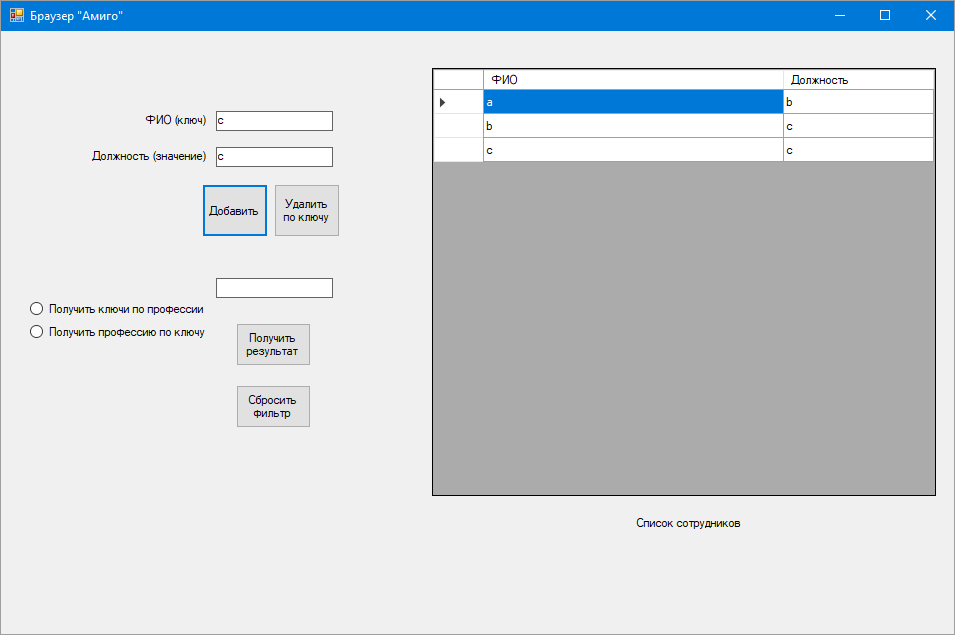
\includegraphics[scale=0.4]{task7/result3.png}
    \caption{Состояние приложения после добавление нескольких элементов по ключу}
    \label{fig:exec7}
\end{figure}
Ниже приведен пример работы программы:
После запуска приложения открывается следующее окно (см. рисунки \ref{fig:result7},\ref{fig:result71})
\begin{figure}[H]
    \centering
    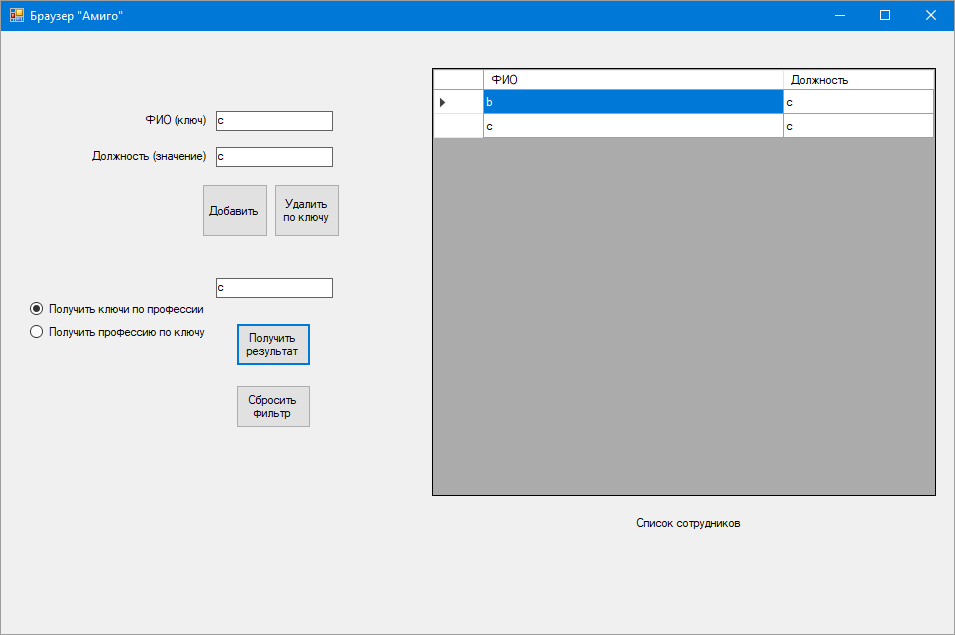
\includegraphics[scale=0.4]{task7/result4.png}
    \caption{Результат поиска по значению}
    \label{fig:result7}
\end{figure}
\begin{figure}[H]
    \centering
    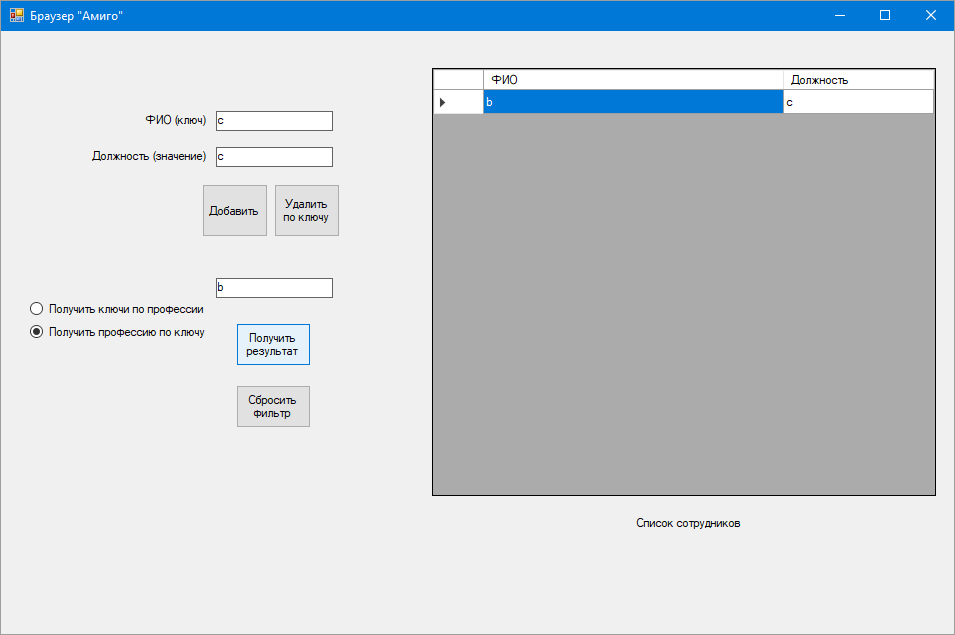
\includegraphics[scale=0.4]{task7/result5.png}
    \caption{Результат поиска по ключу}
    \label{fig:result71}
\end{figure}
В случае, если соответствующие поля не заполнены, выполнение программы
игнорируется.

Полный код программы приведен в приложении \ref{app:repos}.


\section{Файловые диалоги и работа с файлами}

\textbf{Задание:} Создать таблицу Work. В другой файл вывести данные о рабочих, занимающих данную должность. (Вариант 14)

Вид окна представлен на рисунке \ref{fig:task8_form}.
\begin{figure}[H]
    \centering
    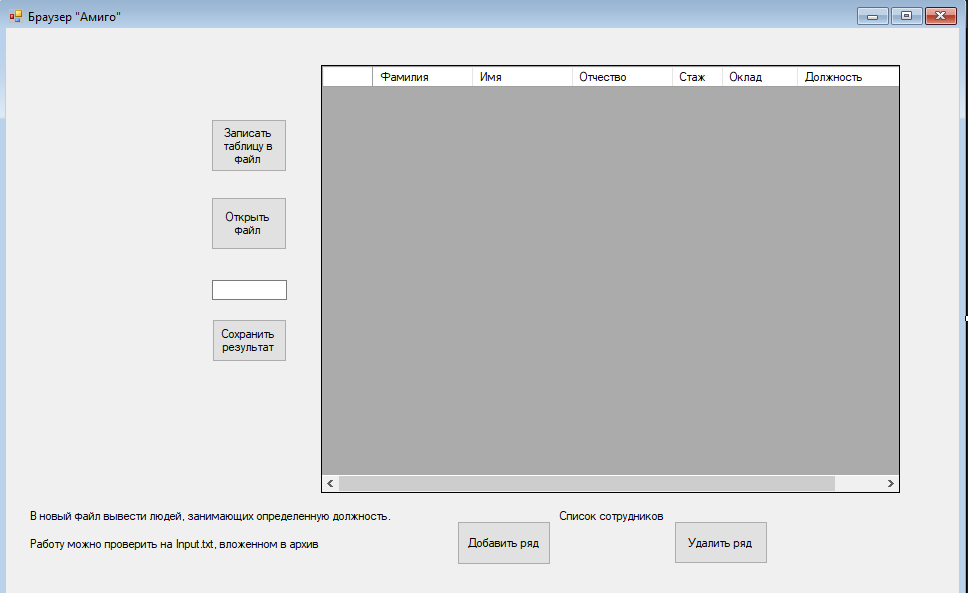
\includegraphics[scale=0.7]{task8/form.png}
    \caption{Внешний вид формы программы}
    \label{fig:task8_form}
\end{figure}
У элементов изменены значения некоторых атрибутов. 
Значения измененных атрибутов представлены в таблице \ref{table:params8}.
\begin{longtable}{|l|l|}
    Наименование атрибута & Значение\cr\hline
    \multicolumn{2}{|l|}{Для формы}\cr\hline
    \verb"Text" & \verb"Браузер "Амиго""\cr\hline
    \verb"FormBorderStyle" & \verb"FixedSingle"\cr\hline
    \verb"MaximizeBox" & \verb"False"\cr\hline
    \multicolumn{2}{|l|}{Для таблицы}\cr\hline
    \verb"(Name)" & \verb"gridResult"\cr\hline
    \multicolumn{2}{|l|}{Для кнопки записи в файл}\cr\hline
    \verb"(Name)" & \verb"SaveFileBtn"\cr\hline
    \multicolumn{2}{|l|}{Для кнопки открытия файла}\cr\hline
    \verb"(Name)" & \verb"OpenFileBtn"\cr\hline
    \multicolumn{2}{|l|}{Для кнопки сохранения результата}\cr\hline
    \verb"(Name)" & \verb"ResultBtn"\cr\hline
    \multicolumn{2}{|l|}{Для текстового поля должности}\cr\hline
    \verb"(Name)" & \verb"ResultTextBox"\cr\hline
    \multicolumn{2}{|l|}{Для обработчика ошибок}\cr\hline
    \verb"(Name)" & \verb"errorProvider1"\cr\hline

    \caption{Значения атрибутов элементов в приложении <<Работа с файлами>>}
    \label{table:params8}
\end{longtable}
Кроме того, это приложение содержит элементы \verb|openFileDialogue|
и \verb|saveFileDialogue|, реализующие открытие и сохранение файлов.

Работа с ними производится в кнопках. Ниже приведен пример работы
функции открытия файла:
\begin{minted}[fontsize=\footnotesize, breaklines=true, style=bw, linenos]{cpp}
private: System::Void OpenFileBtn_Click(System::Object^ sender, System::EventArgs^ e) {
	System::IO::Stream^ myStream;
	if (this->openFileDialog->ShowDialog() == System::Windows::Forms::DialogResult::OK) {
		CreateEmptyMatrix(gridResult, 1);
		if ((myStream = openFileDialog->OpenFile()) != nullptr) {
			System::IO::StreamReader^ sw = gcnew System::IO::StreamReader(myStream, System::Text::Encoding::
			GetEncoding(65001)); // UTF-8
			System::String^ s = "";
			int innerIdx = 0;
			while ((s = sw->ReadLine()) != nullptr && s != "") {
				gridResult->Rows->Add(1);
				int idx = 0;
				int current = 0;
				while (idx != s->Length) { 
					System::String^ currentWord = "";
					while (idx < s->Length && s[idx] != ' ') {
						currentWord += s[idx++];
					}
					if (idx < s->Length && s[idx] == ' ') ++idx;
					gridResult->Rows[innerIdx]->Cells[current++]->Value = currentWord;
					currentWord = "";
				}
				++innerIdx;
			}
		sw->Close();
		}
	}
}
\end{minted}

После запуска программы на экране появляется окно следующего вида (см. рисунок \ref{fig:exec8})
\begin{figure}[H]
    \centering
    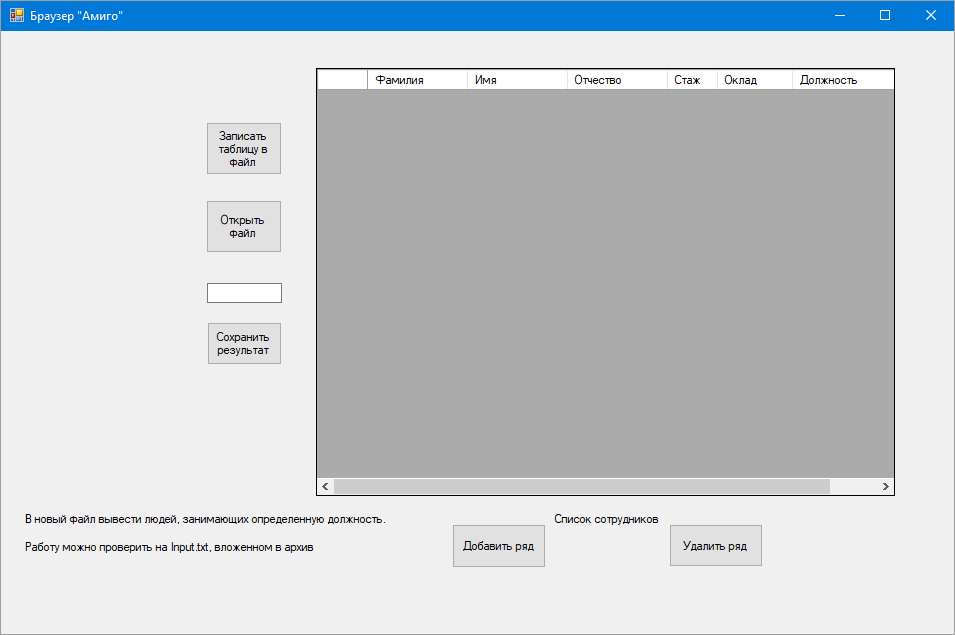
\includegraphics[scale=0.4]{task8/exec.png}
    \caption{Внешний вид окна приложения}
    \label{fig:exec8}
\end{figure}

После открытия файла состояние программы изменится на следующее (см. рисунок \ref{fig:openFile})
\begin{figure}[H]
    \centering
    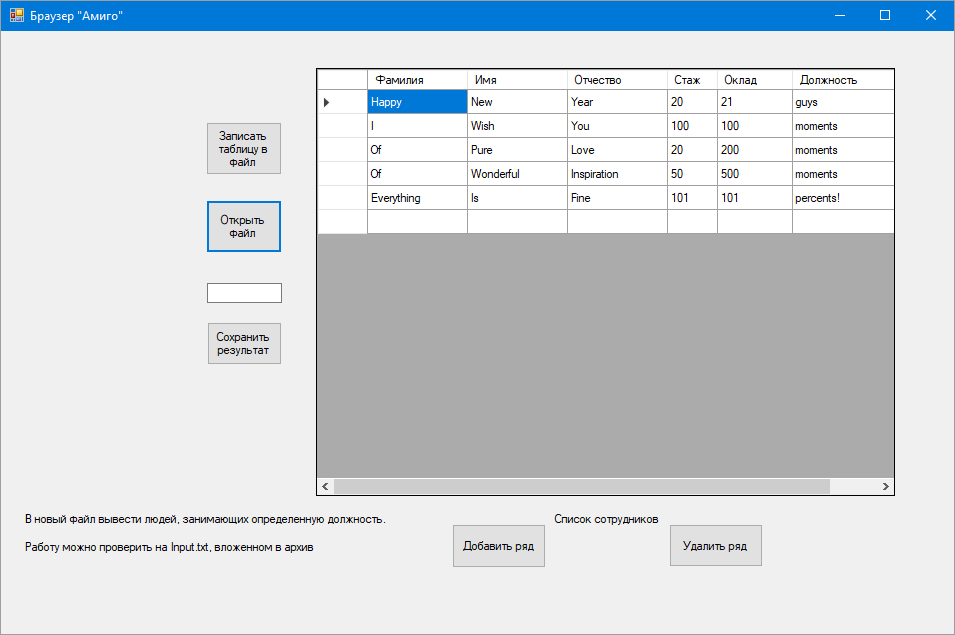
\includegraphics[scale=0.4]{task8/openFile.png}
    \caption{Состояние программы после открытия файла}
    \label{fig:openFile}
\end{figure}

Результатом работы программы является новый файл (см. рисунок \ref{fig:result8})
\begin{figure}[H]
    \centering
    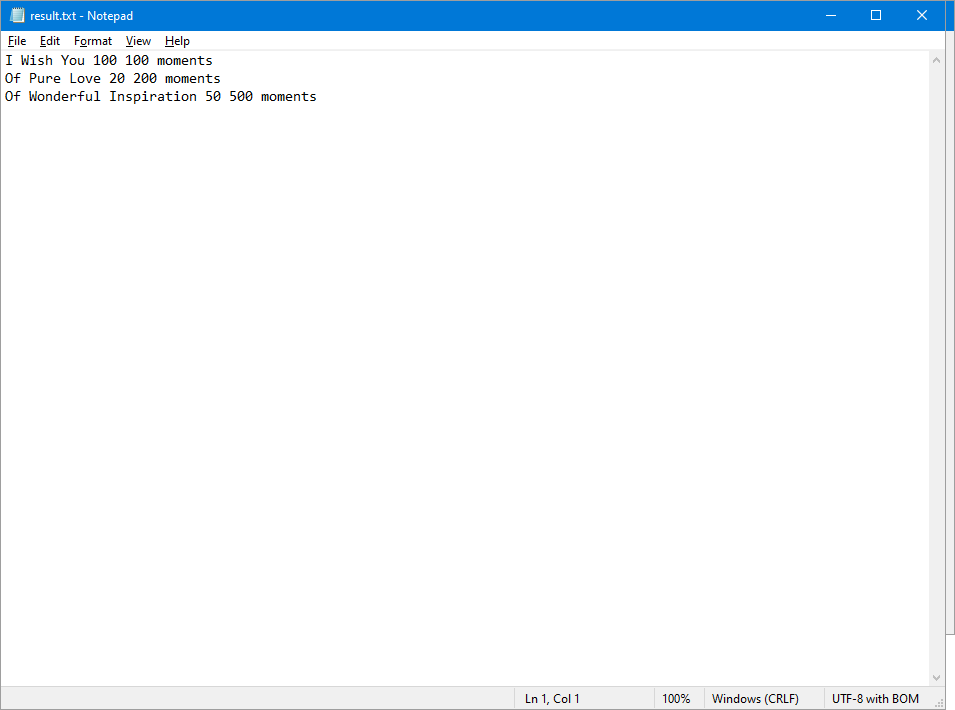
\includegraphics[scale=0.4]{task8/result.png}
    \caption{Результат работы программы}
    \label{fig:result8}
\end{figure}
Возникновение исключительных ситуаций ограничено интерфейсом, постановкой задачи
и программными средствами \verb|.NET framework|.

Полный код программы приведен в приложении \ref{app:repos}.


\section{Приложение <<Тест>>}

\textbf{Задание:} Создать приложение для проведения тестирования. Оно должно содержать:

\begin{enumerate}
    \item Набор вопросов по какой-то теме (и вопросы и ответы должны быть реальные) -не менее 10
    \item Вопросы должны выбираться случайным образом.
    \item Вопросы должны быть нескольких типов - "Да/нет", Выбор одного ответа, Выбор нескольких ответов, Короткий ответ.
    \item Необходимо создать сообщения для правильного и неправильного ответа (Молодец, Не правильно и т.д.)
    \item Необходимо подсчитать количество правильных ответов и вывести результат.
\end{enumerate}
Вид окна представлен на изображениях \ref{fig:task9_form1},\ref{fig:task9_form2}.
\begin{figure}[H]
    \centering
    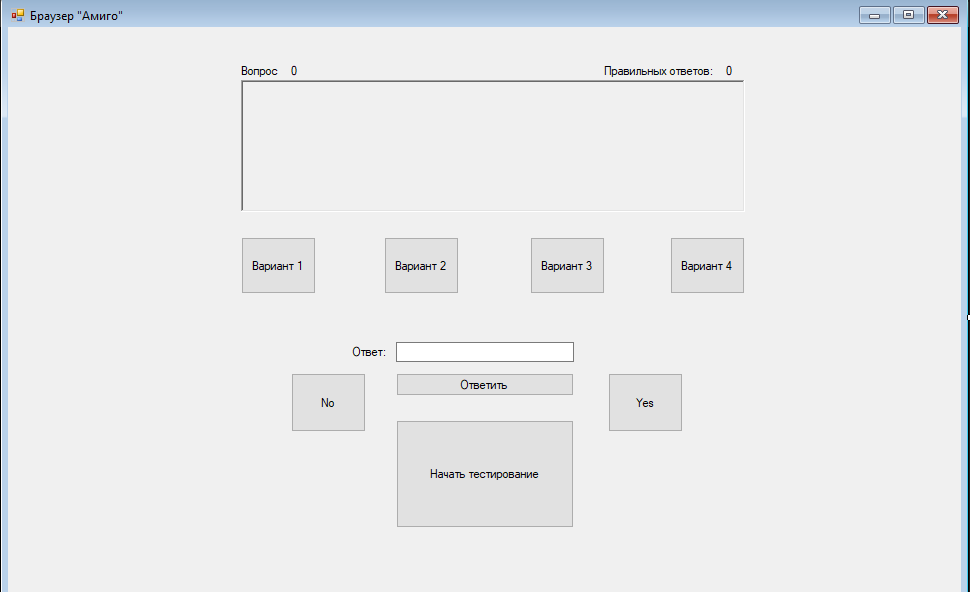
\includegraphics[scale=0.6]{task9/form1.png}
    \caption{Внешний вид формы 1}
    \label{fig:task9_form1}
\end{figure}
\begin{figure}[H]
    \centering
    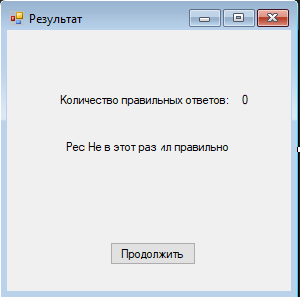
\includegraphics[scale=0.8]{task9/form2.png}
    \caption{Внешний вид формы 2}
    \label{fig:task9_form2}
\end{figure}
У элементов изменены значения некоторых атрибутов. 
Значения измененных атрибутов представлены в таблице \ref{table:params9}.
\begin{longtable}{|l|l|}
    Наименование атрибута & Значение\cr\hline
    \multicolumn{2}{|l|}{Для формы}\cr\hline
    \verb"Text" & \verb"Браузер "Амиго""\cr\hline
    \verb"FormBorderStyle" & \verb"FixedSingle"\cr\hline
    \verb"MaximizeBox" & \verb"False"\cr\hline
    \multicolumn{2}{|l|}{Для кнопки варианта 1}\cr\hline
    \verb"(Name)" & \verb"Option1Btn"\cr\hline
    \verb"Text" & \verb"Вариант 1"\cr\hline
    \multicolumn{2}{|l|}{Для кнопки варианта 2}\cr\hline
    \verb"(Name)" & \verb"Option2Btn"\cr\hline
    \verb"Text" & \verb"Вариант 2"\cr\hline
    \multicolumn{2}{|l|}{Для кнопки варианта 3}\cr\hline
    \verb"(Name)" & \verb"Option3Btn"\cr\hline
    \verb"Text" & \verb"Вариант 3"\cr\hline
    \multicolumn{2}{|l|}{Для кнопки варианта 4}\cr\hline
    \verb"(Name)" & \verb"Option4Btn"\cr\hline
    \verb"Text" & \verb"Вариант 4"\cr\hline
    \multicolumn{2}{|l|}{Для кнопки "Да"}\cr\hline
    \verb"(Name)" & \verb"YesBtn"\cr\hline
    \verb"Text" & \verb"Да"\cr\hline
    \multicolumn{2}{|l|}{Для кнопки "Нет"}\cr\hline
    \verb"(Name)" & \verb"NoBtn"\cr\hline
    \verb"Text" & \verb"Нет"\cr\hline
    \caption{Значения атрибутов элементов в приложении <<Приложение <<Тест>> >>}
    \label{table:params9}
\end{longtable}
После запуска приложения появляется окно (см. рисунок \ref{fig:exec9})
\begin{figure}[H]
    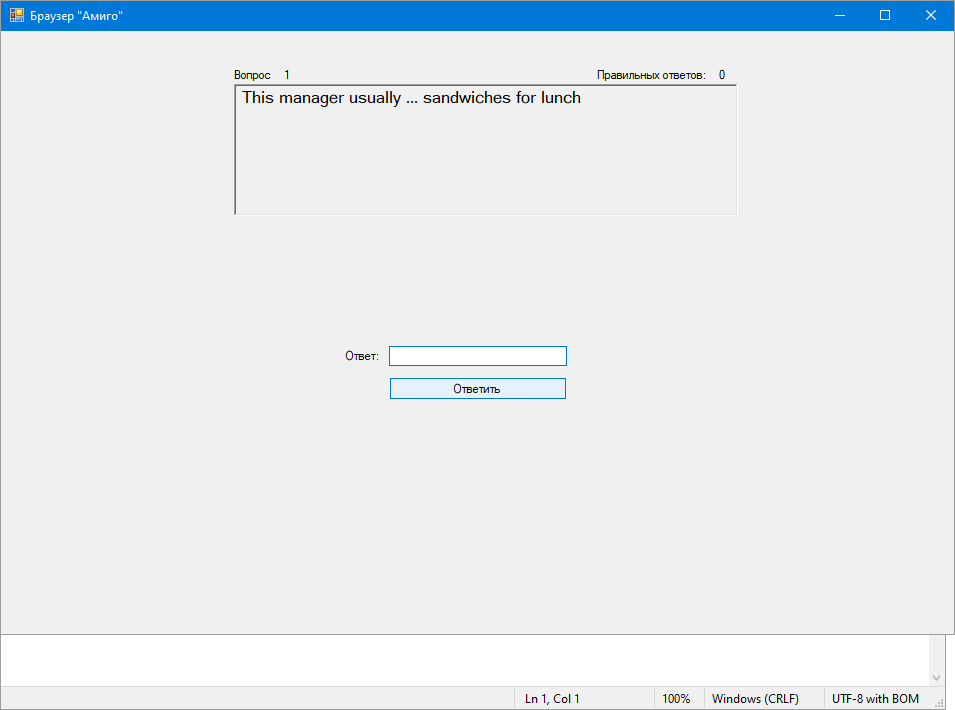
\includegraphics[scale=0.6]{task9/exec.png}
	\caption{Внешний вид окна после запуска приложения}
	\label{fig:exec9}
\end{figure}
Приложение содержит различные виды вопросов. Например, окно для вопросов с двумя вариантами
ответа выглядит следующим образом (см. рисунок \ref{fig:yesorno})
\begin{figure}[H]
    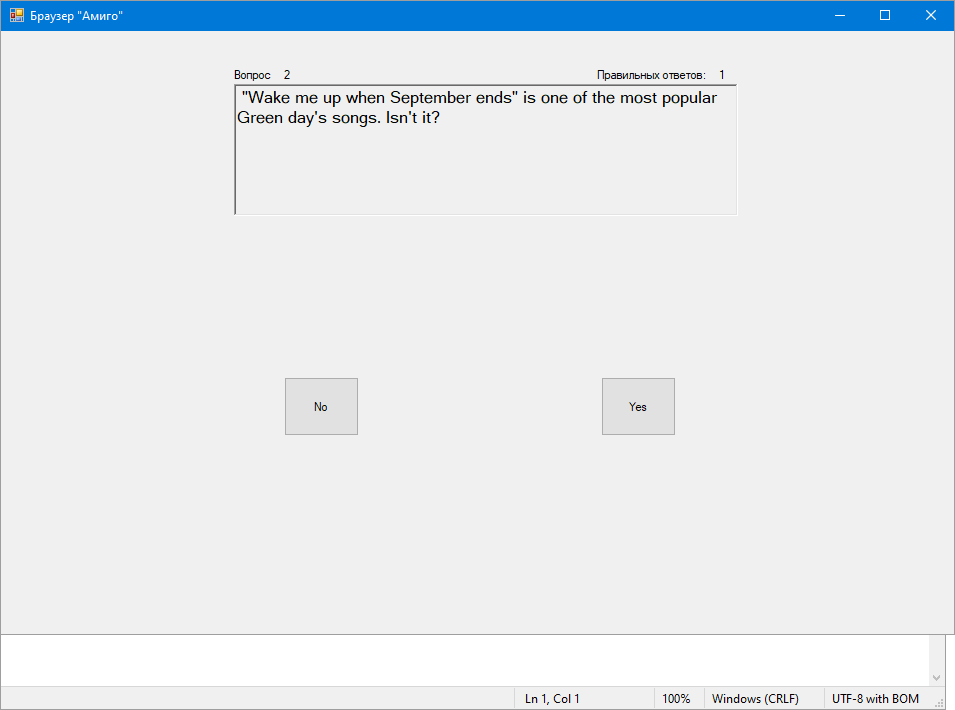
\includegraphics[scale=0.6]{task9/yesorno.png}
	\caption{Внешний вид для вопросов с двумя вариантами ответа}
	\label{fig:yesorno}
\end{figure}
В коде приложения была создана структура наследовования, которая
упрощает работу с различными вариантами вопросов:
\begin{minted}[fontsize=\small, breaklines=true, style=bw, linenos]{cpp}
ref struct Question {
	public: int questionId;
	public: Question() {};
	public: Question(int questionId, String^ text) : questionId(questionId), text(text) {};
	public: String^ text;
	public: virtual bool CheckAnswer() = 0;
	public: virtual Question^ Clone() = 0;
	};

ref struct ShortAnswerQuestion : Question {
	public: String^ expectedAnswer;
	public: String^ userAnswer;
	public: ShortAnswerQuestion() {};
	public: ShortAnswerQuestion(int questionId, String^ expectedAnswer) {
		this->questionId = questionId;
		this->expectedAnswer = expectedAnswer;
	}
	public: virtual bool CheckAnswer() override {
		return expectedAnswer->Equals(userAnswer);
	}
	public: virtual Question^ Clone() override {
		ShortAnswerQuestion^ obj = (gcnew ShortAnswerQuestion());
		obj->expectedAnswer = this->expectedAnswer;
		obj->questionId = this->questionId;
		obj->text = this->text;
		obj->userAnswer = this->userAnswer;
	Question^ toBeReturned = obj;
	return toBeReturned;
	}
};

ref struct SeveralAnswerQuestion : Question {
	public: int count;
	public: int userAnswerId;
	public: int expectedAnswerId;
	public: virtual bool CheckAnswer() override {
		return userAnswerId == expectedAnswerId;
	}
	public: SeveralAnswerQuestion() {};
	public: SeveralAnswerQuestion(int questionId, int expectedAnswer, int count) {
		this->questionId = questionId;
		this->expectedAnswerId = expectedAnswerId;
		this->count = count;
	}
	public: virtual Question^ Clone() override {
		SeveralAnswerQuestion^ obj = (gcnew SeveralAnswerQuestion());
		obj->expectedAnswerId = this->expectedAnswerId;
		obj->questionId = this->questionId;
		obj->text = this->text;
		obj->count = this->count;
		Question^ toBeReturned = obj;
		return toBeReturned;
	}
};
\end{minted}
В ходе выполнения программа сообщает пользователю о том, ввел 
ли он правильный ответ или нет (см. рисунки \ref{fig:whoops},\ref{fig:result9})
\begin{figure}[H]
    \centering
    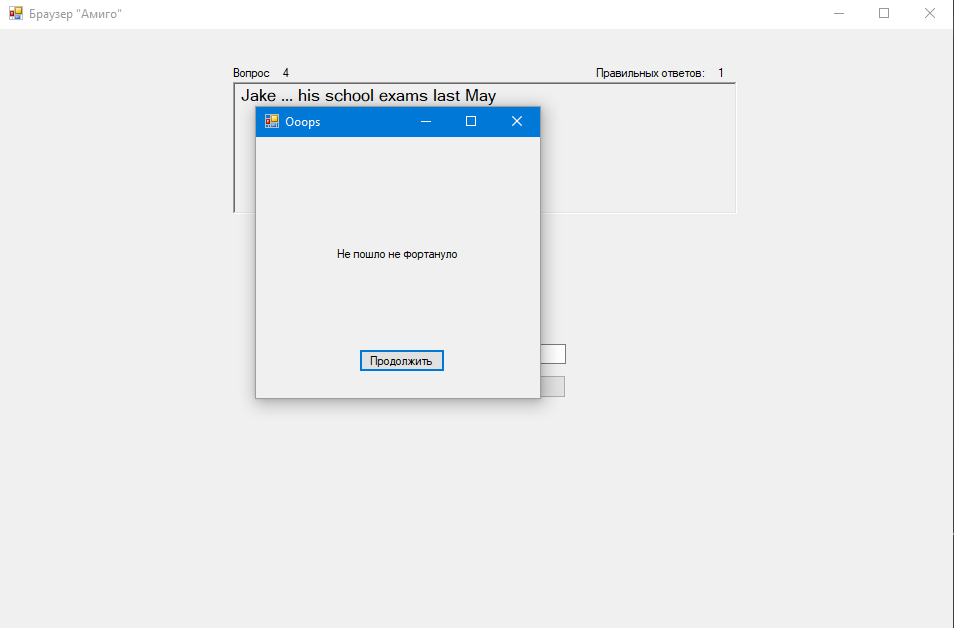
\includegraphics[scale=0.6]{task9/whoops.png}
	\caption{Окно в случае неправильного ответа на вопрос}
	\label{fig:whoops}
\end{figure}
\begin{figure}[H]
    \centering
    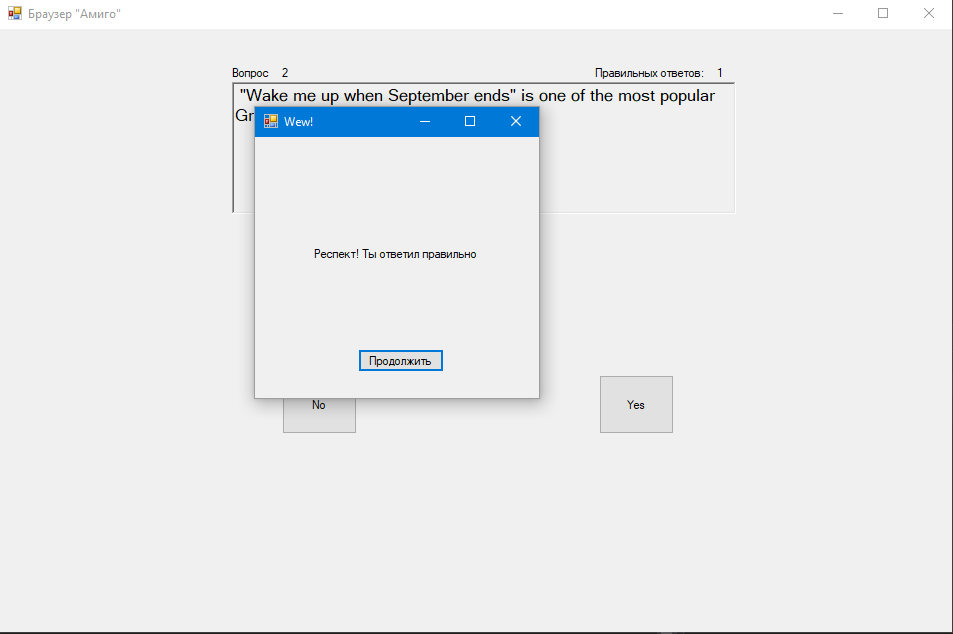
\includegraphics[scale=0.6]{task9/result.png}
	\caption{Окно в случае правильного ответа на вопрос}
	\label{fig:result9}
\end{figure}
Программа не содержит исключительных ситуаций, поэтому в их обработке нет необходимости.

Полный код программы приведен в приложении \ref{app:repos}.



\conclusion

В ходе прохождения практики были получены основы разработки приложений
Windows Forms. Были изучены особенности и основные инструменты
\verb|.NET framework|.

\appendix

\section{Репозиторий Github, содержащий полный код программ}\label{app:repos}

\href{https://github.com/WrongWayboyyyy/StudyPracticePublic}{https://github.com/WrongWayboyyyy/StudyPracticePublic}

\begin{desciption}
	\item \verb|\task1| "--- <<Вычисление факториала>>
	\item \verb|\task2| "--- <<Простые вычисления>>
	\item \verb|\task3| "--- <<Рекурсивные вычисления>>
	\item \verb|\task4| "--- <<Обработка табличных данных. Часть 1>>
	\item \verb|\task5| "--- <<Обработка табличных данных. Часть 2>>
	\item \verb|\task6| "--- <<Матричный калькулятор>>
	\item \verb|\task7| "--- <<Использование коллекций>>
	\item \verb|\task8| "--- <<Файловые диалоги и работа с файлами>>
	\item \verb|\task9| "--- <<Приложение <<Тест>>>>
	\item \verb|practice.pdf| "--- PDF"=файл отчета
\end{desciption}
%Библиографический список, составленный вручную, без использования BibTeX
%
%\begin{thebibliography}{99}
%  \bibitem{Ione} Источник 1.
%  \bibitem{Itwo} Источник 2
%\end{thebibliography}

%Библиографический список, составленный с помощью BibTeX
%
\bibliographystyle{gost780uv}
\bibliography{thesis}

% % При использовании biblatex вместо bibtex
%\printbibliography

% Окончание основного документа и начало приложений
% Каждая последующая секция документа будет являться приложением
\appendix

\end{document}